%%
% The BIThesis Template for Bachelor Graduation Thesis
%
% 北京理工大学毕业设计(论文) —— 使用 XeLaTeX 编译
%
% Copyright 2020 Spencer Woo
%
% This work may be distributed and/or modified under the
% conditions of the LaTeX Project Public License, either version 1.3
% of this license or (at your option) any later version.
% The latest version of this license is in
%   http://www.latex-project.org/lppl.txt
% and version 1.3 or later is part of all distributions of LaTeX
% version 2005/12/01 or later.
%
% This work has the LPPL maintenance status `maintained'.
%
% The Current Maintainer of this work is Spencer Woo.
%
% Compile with: xelatex -> biber -> xelatex -> xelatex

% 章节支持、单面打印:ctexbook
\documentclass[bachelor]{bitbook}
\usepackage[ruled,vlined]{algorithm2e}
% 参考文献引用文件位于 misc/ref.bib
\addbibresource{misc/ref.bib}

% 在这里填写你的论文中英文题目
\newcommand{\thesisTitle}{北京理工大学本科生毕业设计(论文)题目}
\newcommand{\thesisTitleEN}{The Subject of Undergraduate Graduation Project (Thesis) of Beijing Institute of Technology}

% 在这里填写你的相关信息
\newcommand{\deptName}{计算机学院}
\newcommand{\majorName}{计算机科学与技术}
\newcommand{\yourName}{崔程远}
\newcommand{\yourStudentID}{1120171189}
\newcommand{\mentorName}{郑宏}
% 如果你的毕设为校外毕设,请将下面这一行语句解除注释(删除第一个百分号字符)并在第二组花括号中填写你的校外毕设导师名字
% \newcommand{\externalMentorName}{左偏树}

% 文档开始
\begin{document}

% 标题页面:如无特殊需要,本部分无需改动
%%
% The BIThesis Template for Bachelor Graduation Thesis
%
% 北京理工大学毕业设计(论文)封面页 —— 使用 XeLaTeX 编译
%
% Copyright 2020 Spencer Woo
%
% This work may be distributed and/or modified under the
% conditions of the LaTeX Project Public License, either version 1.3
% of this license or (at your option) any later version.
% The latest version of this license is in
%   http://www.latex-project.org/lppl.txt
% and version 1.3 or later is part of all distributions of LaTeX
% version 2005/12/01 or later.
%
% This work has the LPPL maintenance status `maintained'.
%
% The Current Maintainer of this work is Spencer Woo.
%
% 封面
%
% 如无特殊需要,本页面无需更改

% Underline new command for student information
% Usage: \dunderline[<offset>]{<line_thickness>}
\newcommand\dunderline[3][-1pt]{{%
  \setbox0=\hbox{#3}
  \ooalign{\copy0\cr\rule[\dimexpr#1-#2\relax]{\wd0}{#2}}}}

% Cover Page
\begin{titlepage}
  \makeatletter
  \@ifundefined{externalMentorName}{
    % 校内毕设封面顶部间距
    \vspace*{19mm}
  }{
    % 校外毕设封面顶部间距
    \vspace*{13mm}
  }
  \centering

  
\includegraphics[width=9.87cm]{images/header.png}

  \vspace*{-3mm}

  \zihao{-0}\textbf{\ziju{0.12}\songti{本科生毕业设计(论文)}}

  \vspace{16mm}

  \zihao{2}\textbf{\xihei\thesisTitle}

  \vspace{3mm}

  \begin{spacing}{1.2}
    \zihao{3}\selectfont{\textbf{\thesisTitleEN}}
  \end{spacing}

  \vspace{15mm}

  \flushleft

  \makeatletter
  \@ifundefined{externalMentorName}{
    % 生成校内毕设封面字段
    \makeatother
    \begin{spacing}{1.8}
      \hspace{27mm}\songti\zihao{3}\selectfont{学\hspace{11mm}院:\dunderline[-10pt]{1pt}{\makebox[78mm][c]{\deptName}}}

      \hspace{27mm}\songti\zihao{3}\selectfont{专\hspace{11mm}业:\dunderline[-10pt]{1pt}{\makebox[78mm][c]{\majorName}}}

      \hspace{27mm}\songti\zihao{3}\selectfont{学生姓名:\dunderline[-10pt]{1pt}{\makebox[78mm][c]{\yourName}}}

      \hspace{27mm}\songti\zihao{3}\selectfont{学\hspace{11mm}号:\dunderline[-10pt]{1pt}{\makebox[78mm][c]{\yourStudentID}}}

      \hspace{27mm}\songti\zihao{3}\selectfont{指导教师:\dunderline[-10pt]{1pt}{\makebox[78mm][c]{\mentorName}}}
    \end{spacing}
  }{
    % 生成校外毕设封面字段
    \makeatother
    \begin{spacing}{1.8}
      \hspace{19.4mm}\songti\zihao{3}\selectfont{学\hspace{19.6mm}院\hspace{3mm}:\dunderline[-10pt]{1pt}{\makebox[77.4mm][c]{\deptName}}}

      \hspace{19.4mm}\songti\zihao{3}\selectfont{专\hspace{19.6mm}业\hspace{3mm}:\dunderline[-10pt]{1pt}{\makebox[77.4mm][c]{\majorName}}}

      \hspace{19.4mm}\songti\zihao{3}\selectfont{学\hspace{2.8mm}生\hspace{2.8mm}姓\hspace{2.8mm}名\hspace{3mm}:\dunderline[-10pt]{1pt}{\makebox[77.4mm][c]{\yourName}}}

      \hspace{19.4mm}\songti\zihao{3}\selectfont{学\hspace{19.6mm}号\hspace{3mm}:\dunderline[-10pt]{1pt}{\makebox[77.4mm][c]{\yourStudentID}}}

      \hspace{19.4mm}\songti\zihao{3}\selectfont{指\hspace{2.8mm}导\hspace{2.8mm}教\hspace{2.8mm}师\hspace{3mm}:\dunderline[-10pt]{1pt}{\makebox[77.4mm][c]{\mentorName}}}

      \hspace{19.4mm}\songti\zihao{3}\selectfont{校外指导教师:\dunderline[-10pt]{1pt}{\makebox[77.4mm][c]{\externalMentorName}}}
    \end{spacing}
  }

  \vspace{25mm}
  \centering
  \zihao{3}\ziju{0.5}\songti{\today}
\end{titlepage}


% 前置页面定义
\frontmatter
% 原创性声明:如无特殊需要,本部分无需改动
% 更改为 PDF 页面插入,如需要添加内容,可考虑先用 Word 制作再覆盖 misc/1_originality.pdf
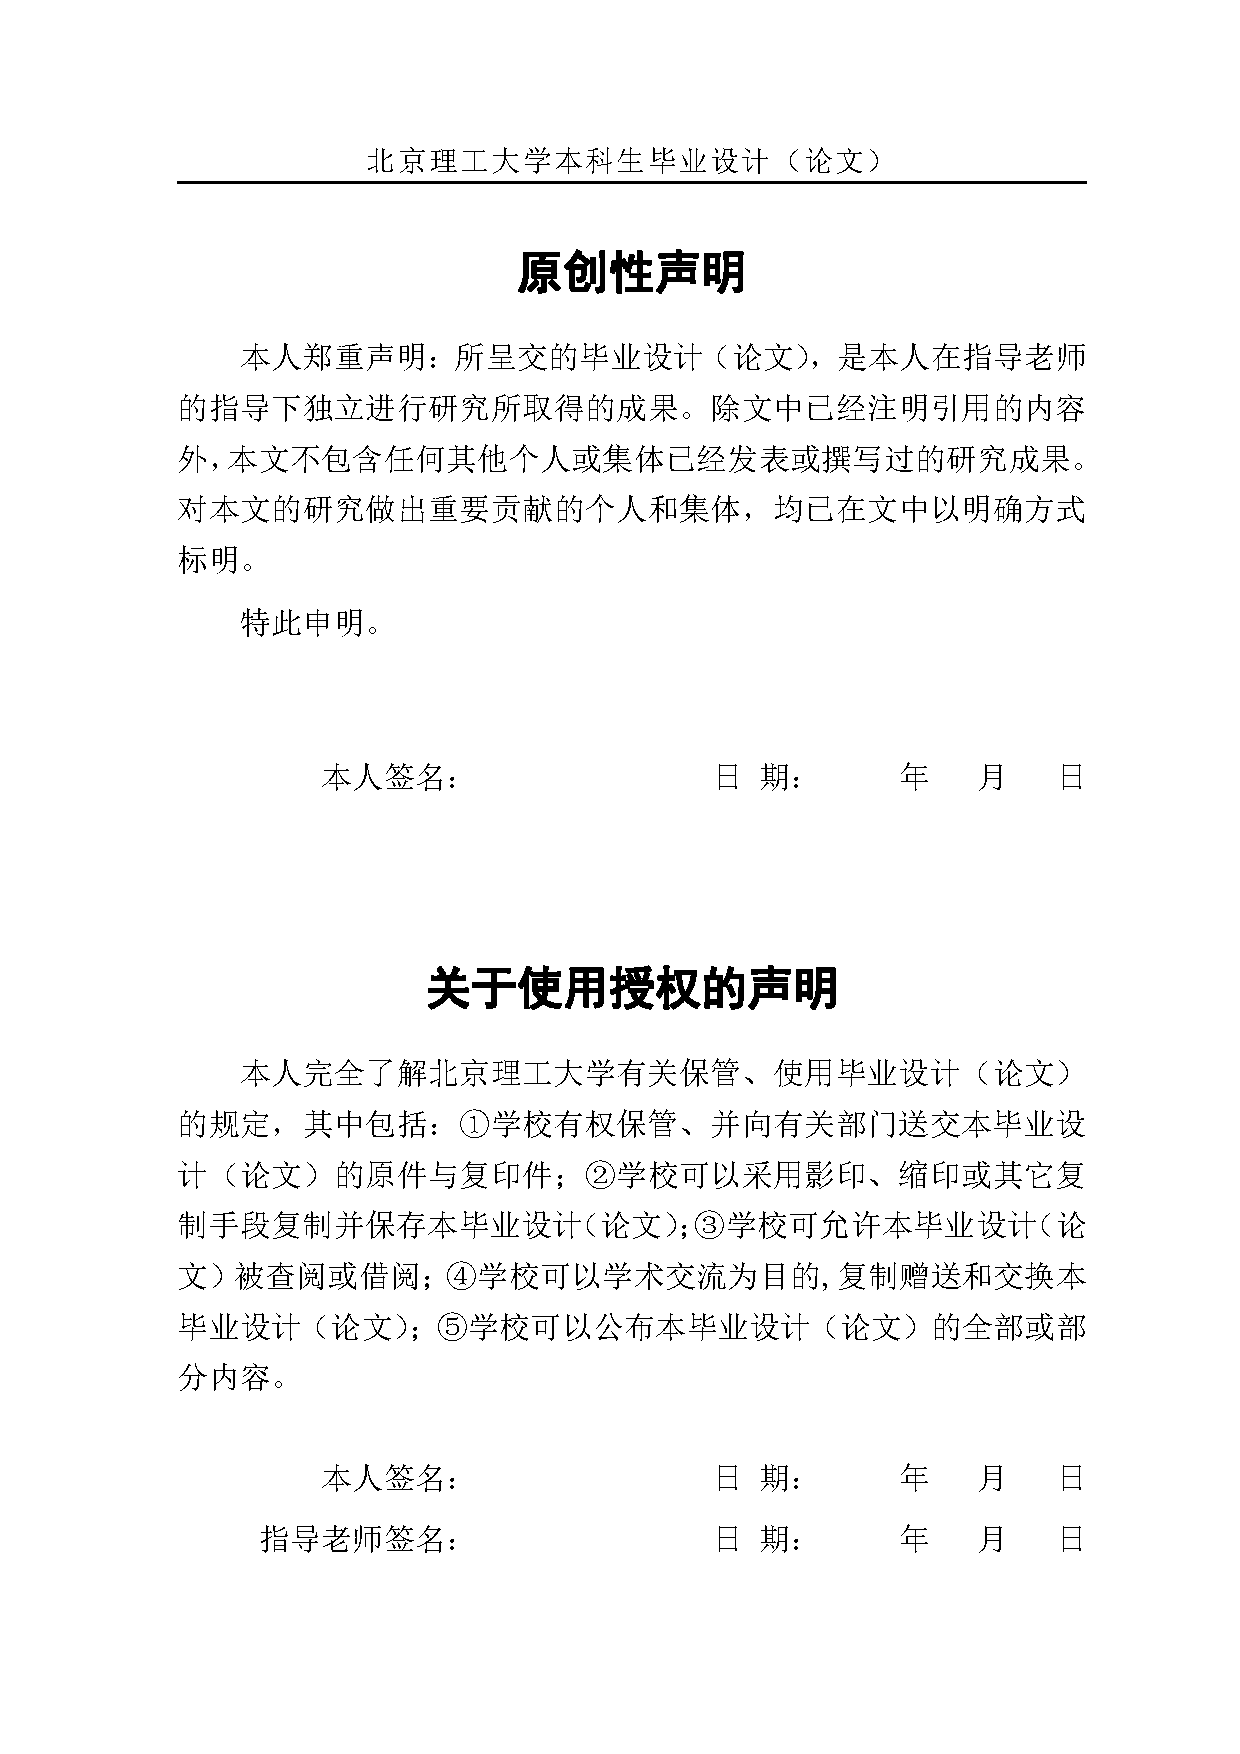
\includepdf{misc/1_originality.pdf}
\newpage
%%%
% The BIThesis Template for Bachelor Graduation Thesis
%
% 北京理工大学毕业设计(论文)原创性声明页 —— 使用 XeLaTeX 编译
%
% Copyright 2020 Spencer Woo
%
% This work may be distributed and/or modified under the
% conditions of the LaTeX Project Public License, either version 1.3
% of this license or (at your option) any later version.
% The latest version of this license is in
%   http://www.latex-project.org/lppl.txt
% and version 1.3 or later is part of all distributions of LaTeX
% version 2005/12/01 or later.
%
% This work has the LPPL maintenance status `maintained'.
%
% The Current Maintainer of this work is Spencer Woo.
%
% 如无特殊需要,本页面无需更改

% 原创性声明页无页码页面格式
\fancypagestyle{originality}{
  % 页眉高度
  \setlength{\headheight}{20pt}

  % 页眉和页脚(页码)的格式设定
  \fancyhf{}
  \fancyhead[C]{\zihao{4}\ziju{0.08}\songti{北京理工大学本科生毕业设计(论文)}}

  % 页眉分割线稍微粗一些
  \renewcommand{\headrulewidth}{0.6pt}
}

\pagestyle{originality}
\topskip=0pt

% 圆形数字编号定义
\newcommand{\circled}[2][]{\tikz[baseline=(char.base)]
  {\node[shape = circle, draw, inner sep = 1pt]
  (char) {\phantom{\ifblank{#1}{#2}{#1}}};
  \node at (char.center) {\makebox[0pt][c]{#2}};}}
\robustify{\circled}

% 设置行间距
\setlength{\parskip}{0.4em}
\renewcommand{\baselinestretch}{1.41}

% 顶部空白
\vspace*{-6mm}

% 原创性声明部分
\begin{center}
  \heiti\zihao{2}\textbf{原创性声明}
\end{center}

% 本部分字号为小三
\zihao{-3}

本人郑重声明:所呈交的毕业设计(论文),是本人在指导老师的指导下独立进行研究所取得的成果。除文中已经注明引用的内容外,本文不包含任何其他个人或集体已经发表或撰写过的研究成果。对本文的研究做出重要贡献的个人和集体,均已在文中以明确方式标明。

特此申明。

\vspace{13mm}

\begin{flushright}
  本人签名:\hspace{40mm}日\hspace{2.5mm}期:\hspace{13mm}年\hspace{8mm}月\hspace{8mm}日
\end{flushright}

\vspace{17mm}

% 使用授权声明部分
\begin{center}
  \heiti\zihao{2}\textbf{关于使用授权的声明}
\end{center}

本人完全了解北京理工大学有关保管、使用毕业设计(论文)的规定,其中包括:\circled{1}学校有权保管、并向有关部门送交本毕业设计(论文)的原件与复印件;\circled{2}学校可以采用影印、缩印或其它复制手段复制并保存本毕业设计(论文);\circled{3}学校可允许本毕业设计(论文)被查阅或借阅;\circled{4}学校可以学术交流为目的,复制赠送和交换本毕业设计(论文);\circled{5}学校可以公布本毕业设计(论文)的全部或部分内容。

\vspace*{1mm}

\begin{flushright}
  \begin{spacing}{1.65}
    \zihao{-3}
    本人签名:\hspace{40mm}日\hspace{2.5mm}期:\hspace{13mm}年\hspace{8mm}月\hspace{8mm}日\\
    指导老师签名:\hspace{40mm}日\hspace{2.5mm}期:\hspace{13mm}年\hspace{8mm}月\hspace{8mm}日
  \end{spacing}
\end{flushright}

\newpage

% 摘要:在摘要相应的 TeX 文件处进行摘要部分的撰写
%%
% The BIThesis Template for Bachelor Graduation Thesis
%
% 北京理工大学毕业设计(论文)中英文摘要 —— 使用 XeLaTeX 编译
%
% Copyright 2020 Spencer Woo
%
% This work may be distributed and/or modified under the
% conditions of the LaTeX Project Public License, either version 1.3
% of this license or (at your option) any later version.
% The latest version of this license is in
%   http://www.latex-project.org/lppl.txt
% and version 1.3 or later is part of all distributions of LaTeX
% version 2005/12/01 or later.
%
% This work has the LPPL maintenance status `maintained'.
%
% The Current Maintainer of this work is Spencer Woo.

% 中英文摘要章节
\zihao{-4}
\vspace*{-11mm}

\begin{center}
  \heiti\zihao{-2}\textbf{\thesisTitle}
\end{center}

\vspace*{2mm}

{\let\clearpage\relax \chapter*{\textmd{摘~~~~要}}}
\addcontentsline{toc}{chapter}{摘~~~~要}
\setcounter{page}{1}

\vspace*{1mm}

\setstretch{1.53}
\setlength{\parskip}{0em}

% 中文摘要正文从这里开始
本文……。

\textcolor{blue}{摘要正文选用模板中的样式所定义的“正文”,每段落首行缩进 2 个字符;或者手动设置成每段落首行缩进 2 个汉字,字体:宋体,字号:小四,行距:固定值 22 磅,间距:段前、段后均为 0 行。阅后删除此段。}

\textcolor{blue}{摘要是一篇具有独立性和完整性的短文,应概括而扼要地反映出本论文的主要内容。包括研究目的、研究方法、研究结果和结论等,特别要突出研究结果和结论。中文摘要力求语言精炼准确,本科生毕业设计(论文)摘要建议 300-500 字。摘要中不可出现参考文献、图、表、化学结构式、非公知公用的符号和术语。英文摘要与中文摘要的内容应一致。阅后删除此段。}

\vspace{4ex}\noindent\textbf{\heiti 关键词:北京理工大学;本科生;毕业设计(论文)}
\newpage

% 英文摘要章节
\vspace*{-2mm}

\begin{spacing}{0.95}
  \centering
  \heiti\zihao{3}\textbf{\thesisTitleEN}
\end{spacing}

\vspace*{17mm}

{\let\clearpage\relax \chapter*{
  \zihao{-3}\textmd{Abstract}\vskip -3bp}}
\addcontentsline{toc}{chapter}{Abstract}
\setcounter{page}{2}

\setstretch{1.53}
\setlength{\parskip}{0em}

% 英文摘要正文从这里开始
In order to study……

\textcolor{blue}{Abstract 正文设置成每段落首行缩进 2 字符,字体:Times New Roman,字号:小四,行距:固定值 22 磅,间距:段前、段后均为 0 行。阅后删除此段。}

\vspace{3ex}\noindent\textbf{Key Words: BIT; Undergraduate; Graduation Project (Thesis)}
\newpage

% 目录:如无特殊需要,本部分无需改动
%%
% The BIThesis Template for Bachelor Graduation Thesis
%
% 北京理工大学毕业设计(论文)目录 —— 使用 XeLaTeX 编译
%
% Copyright 2020 Spencer Woo
%
% This work may be distributed and/or modified under the
% conditions of the LaTeX Project Public License, either version 1.3
% of this license or (at your option) any later version.
% The latest version of this license is in
%   http://www.latex-project.org/lppl.txt
% and version 1.3 or later is part of all distributions of LaTeX
% version 2005/12/01 or later.
%
% This work has the LPPL maintenance status `maintained'.
%
% The Current Maintainer of this work is Spencer Woo.
%
% 如无特殊需要,本页面无需更改

% 目录开始

% 调整目录行间距
\renewcommand{\baselinestretch}{1.35}
% 目录
\tableofcontents
\newpage


% 正文开始
\mainmatter
% 正文 22 磅的行距
\setlength{\parskip}{0em}
\renewcommand{\baselinestretch}{1.53}
% 修复脚注出现跨页的问题
\interfootnotelinepenalty=10000

% 第一章
%%
% The BIThesis Template for Bachelor Graduation Thesis
%
% 北京理工大学毕业设计(论文)第一章节 —— 使用 XeLaTeX 编译
%
% Copyright 2020 Spencer Woo
%
% This work may be distributed and/or modified under the
% conditions of the LaTeX Project Public License, either version 1.3
% of this license or (at your option) any later version.
% The latest version of this license is in
%   http://www.latex-project.org/lppl.txt
% and version 1.3 or later is part of all distributions of LaTeX
% version 2005/12/01 or later.
%
% This work has the LPPL maintenance status `maintained'.
%
% The Current Maintainer of this work is Spencer Woo.
%
% 第一章节

\chapter{前言}

\section{系统背景}
奖学金是教务、教学系统中的重要组成部分,对奖学金进行推荐与效果评估对教学管理与学生发展都有重要意义,这其中主要包括两部分的内容:分别是奖学金分配与奖学金评价,在此我将分别进行介绍。

第一部分是如何进行奖学金分配,即以奖学金的规定为标准对奖学金进行分发,我们有两种手段,一种是根据现有的标准对学生的多种指标(成绩、论文、竞赛等)进行数值换算从而得到数值评价并直接按数值顺序等规则颁发奖学金,也就是现在在本科生奖学金颁发中常用的综合测评等评价指标,这种方法主要基于已有的经验公式进行奖学金计算与推荐;第二种则是以学生的获奖、论文、竞赛等为依据以奖学金申请条件为标准进行推荐,这种方法是以推荐系统的思想为基础进行推荐,但是这种推荐与常用的内容、商品推荐等亦有差别,主要体现为内容、商品等信息推荐能够通过用户在平台积累的大量历史数据信息获得较为完整的用户画像,并且平台累积的用户数据丰富,适合进行推荐,而本研究的系统数据量少而且标签分布不均匀,对推荐算法的设计与特征的构建而言是一个较大的困难与挑战。

第二部分是通过学生的历史奖学金记录与其获奖周边历史信息对奖学金效果进行评价,这里就需要对用户进行时序上的画像,那么如何构建评价指标也是比较困难的一个工作,因为衡量效果的指标有多种,包括成绩变化、论文发表、专利申请、竞赛获奖等内容,需要对评价指标进行设计,而这仅仅是数据的标签部分,甚至于数据的标签可能是一个向量输出多维度指标也有可能,训练的特征也需要进行设计才能使模型进行有效的评价,这里可能需要用到时序的神经网络才能实现。这一部分由于本研究的数据量过少且分布不均匀而没有进行实现。所以可以看到在奖学金这个领域相关研究基本处于空白状态。

我同时查询了与奖学金有关的推荐系统,在这个领域基本处于空白状态,与此类似的系统绝大部分集中于对应届生进行工作推荐,如大学生兼职电商平台工作推荐系统的实现\cite{郭洁畅2017大学生兼职电商平台工作推荐系统的实现}、一种面向冷启动学生用户的工作推荐系统及推荐方法\cite{一种面向冷启动学生用户的工作推荐系统及推荐方法}等。国外的相关文献绝大部分也集中于对教学资源的分配与推荐,如EduRecomSys: An Educational Resource Recommender System Based on Collaborative Filtering and Emotion Detection\cite{bustos2020edurecomsys}。

可以看到在奖学金推荐这个领域相关研究基本处于空白状态。

\section{类似系统现状及问题}

推荐的基础是数据,对于一个典型的推荐系统而言,我们可以获得的数据总体来分为三种,分别是用户的信息、物品的信息以及用户的行为信息。所以按照数据来源可以将推荐系统分为基于内容的推荐以及基于用户行为的推荐两类。

总体而言,推荐系统的两大任务可以分为推荐和预测,所以推荐系统实现的评价指标也可以从上述两方面定义,分别是评分预测以及top-N推荐,评分预测的目的就是通过已有的用户评价数据或者用户浏览数据对用户的评价模型进行学习;Top-N推荐是给用户推送一个根据用户浏览历史或者相似度信息匹配得到的包含多个内容项的以推荐列表形式呈现的信息。在我们的系统中我们主要希望实现的是Top-N推荐,从目前已有的数据来看共10种奖学金,系统预期的功能是给目标用户返回一个奖学金列表以提高推荐的成功率,降低用户手工对奖学金进行选择的时间成本,提高奖学金推送的推送效率。

Top-N推荐算法典型的应用场景为商品推荐系统,这也是目前研究、应用比较丰富的一类系统,在Amazon、豆瓣、淘宝、当当等电商、网商平台都有大规模的应用。此类系统中大致有两种思路,一种是基于商品把商品推荐给用户,也就对应于上文中基于内容的推荐,第二种是以用户为基础通过计算用户的相似性将用户推荐给商品,对应于上文中基于人口统计学和用户行为规则的推荐。图\ref{NetEase_Music}即为典型的Top-N个性化推荐系统。

\begin{figure}[htbp]
    \vspace{3pt} % 调整图片与上文的垂直距离
    \centering
    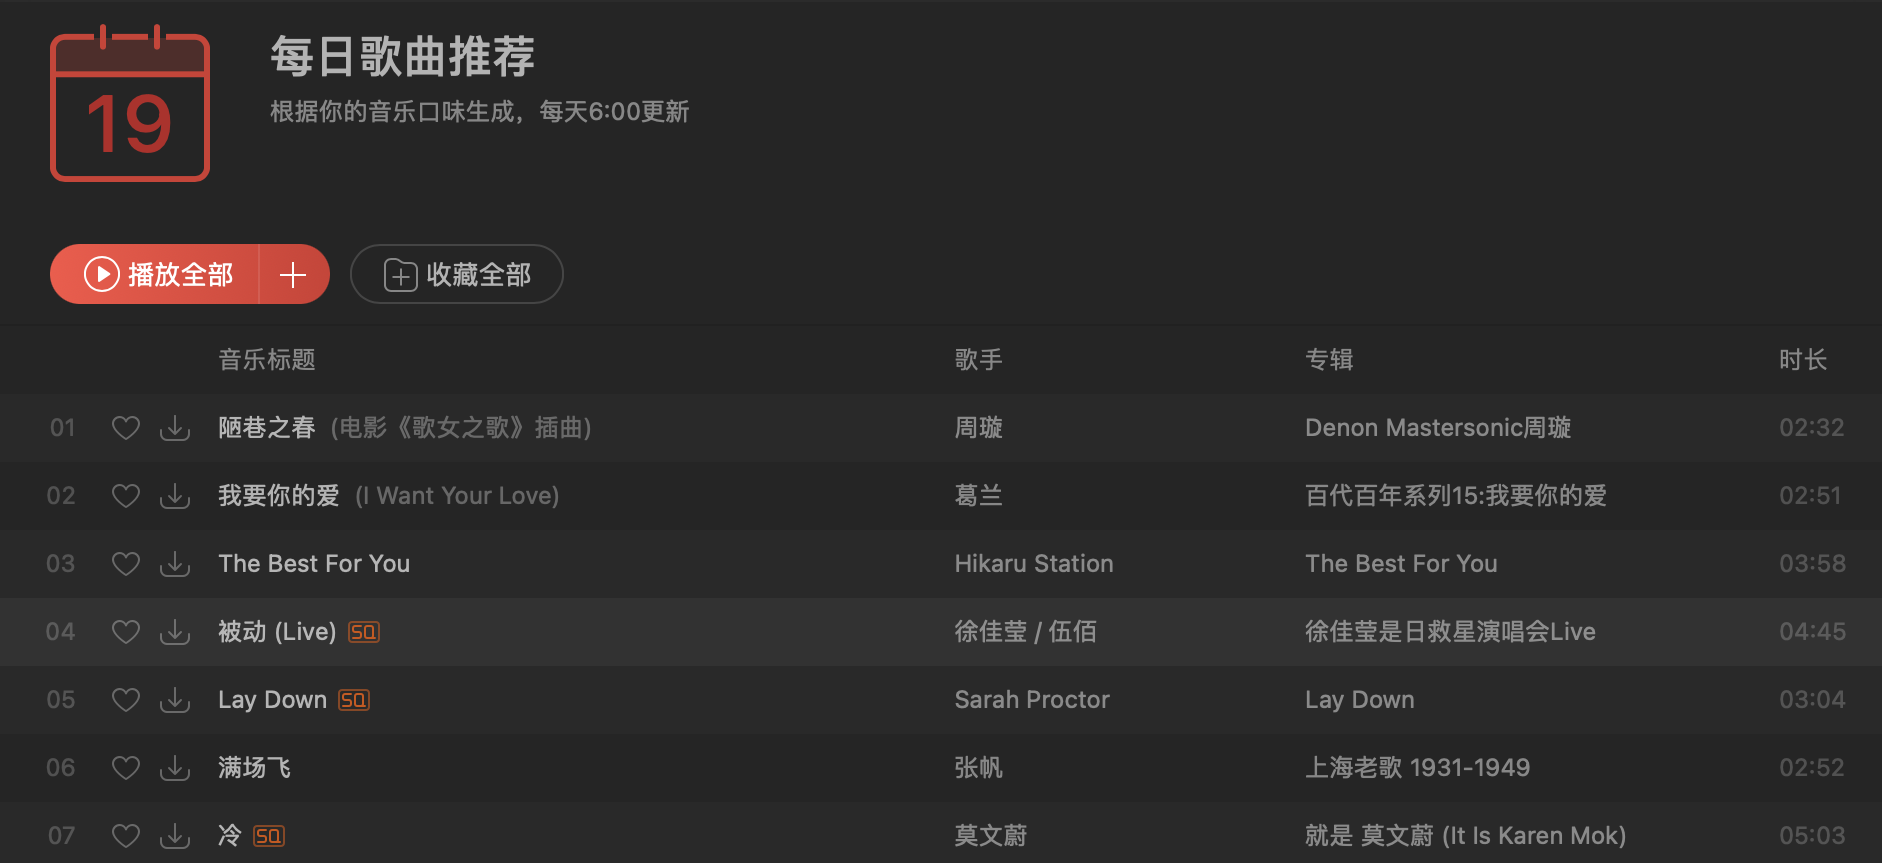
\includegraphics[width=0.9\textwidth]{images/NetEaseMusic.png}
    \caption{网易云音乐歌曲Top-N推荐}\label{NetEase_Music} % label 用来在文中索引
  \end{figure}

Top-N推荐的主要方法包括协同过滤算法(CF)、矩阵分解、因子分解机(Factorization Machines)、逻辑回归、梯度提升决策树(GBDT)、深度神经网络等为代表的一系列模型.

\subsection{传统机器学习模型}

在上述模型中基于协同过滤的推荐(Collaborative Filtering)算法是应用最早和最为成功的技术之一,协同过滤一般分为两大类,分别是基于近邻关系的过滤(neighborhood-based)和基于模型的过滤(model-based)。
其中基于近邻的过滤又可以分为两大类,分别是User-based与Item-based,这两类的区别在于基于用户的过滤原理是利用用户的历史喜好信息计算用户之间的距离,然后利用相似用户的加权商品评分来对目标用户可能的购买行为进行预测,它能够有效的在较少的用户反馈量当中个性化学习其他相似用户的反馈信息\cite{姜保庆2014基于社交网络的一种个性化推荐算法}。

而Item-based的思想为通过计算商品和商品之间的相似度特征获取商品和商品之间的关联矩阵,通过对相似度高的商品进行预测目标用户评分得到用户的购买可能率。在最近邻的加权计算过程与相似度计算过程中,只分析了用户对用户或物品对物品的关系,所以它的运算速度相当快,并且在大型或小型的推荐系统都适用;而基于模型过滤则是最为常见的过滤算法类型,其原理是因为用户存在行为矩阵,用户的行为矩阵与物品之间存在隐变量,算法使用用户行为矩阵经过矩阵分解计算后的低阶用户矩阵和物品矩阵相乘来进行结果预测,其主流方法包括关联、聚类、分类、矩阵分解、神经网络及隐语义模型等。此类模型的推荐效果相对最近邻较好,但是算法训练时间较长复杂度较高使得推荐系统的训练以及在线推荐时间大幅上涨。由于基于模型的原理是用户和物品之间存在隐变量,所以早期推荐系统为了减少运算规模,常用推荐方法还有基于关联规则的推荐,由于用户的购买是存在关联性特征的,所以此类方法的主要思想就是通过算法统计用户的购买倾向,如对购买了商品集合A的用户和商品集合A与商品集合B存在关联的规则对用户推荐集合B中的商品。对于小型的推荐系统而言,使用较多的算法为Item-based的协同过滤算法,而对于大型的系统,由于存在丰富的用户特征以及商品特征,则可以考虑基于用户的协同过滤或基于模型的过滤算法。

但是随着数据量的积累,常用的数据特征工程方法one-hot encoding在面对大规模数据集的时候表现出了难以解决的缺陷,比如在一个有10000商品和1000000用户的系统中如果对用户的商品购买特点进行one-hot encoding那么总的特征空间过大而导致最终的特征矩阵过于稀疏,所以这样对网络的训练而言造成了比较大的困难,而且也导致了很多不必要的存储空间的浪费,所以大数据的高效处理也是一个棘手的问题。对于巨大的特征空间而言,可采用的方法包括使用PCA进行主成分分析降低特征维度,而且在实际应用中one-hot encoding后得到特征向量再经过PCA主成分分析进行降维的组合非常有用。除此以外FM、FFM以及DeepFM等也在此领域大显身手。

\subsection{深度学习模型}

神经网络、机器学习技术的进步协同过滤也有了一些新的思路,其中较为典型的思路包括使用GBDT或XGBoost等集成学习模型进行混合推荐、使用矩阵分解的思路对矩阵进行更快速的降维处理与提取、基于深度学习的协同过滤算法等。

随着深度神经网络在近年的发展,越来越多的模型也选择采用神经网络作为推荐算法进行推荐,典型的算法包括DeepFM、Deep\&Wide等,2016年Google提出的Deep\&wide模型就在YouTube的视频推荐中应用并且取得了不凡的效果,
离线和在线测试相比传统的算法均有较大提高,同时2017年华为联合高校提出了DeepFM的方法,克服了Deep\&Wide需要手工特征工程的缺点结合FM和Deep\&Wide的优点对低阶和高阶特征同时进行学习,训练了一个使用FM+DNN的端到端神经网络。

但是协同过滤算法也包括一些固有的问题,比如典型的冷启动问题与特征空间稀疏问题。这两类问题目前都没有比较好的解决思路。其中冷启动问题在我们的实验数据上也会涉及。但是由于此系统的用户数据量比较少,对应的奖学金(商品)数量也比较少,所以这个问题同样无法适用于常见的冷启动解决思路。

\section{本文主要系统实现}

本文系统主要实现的是基于系统过滤的奖学金推荐算法,数据集来自计算机学院2016级学生以及2017级学生的真实数据,数据集中可用数据的规模在200人左右。在本文中首先进行了数据库架构的构建,然后将保存数据的excel文件转换为sqlite数据库当中的记录,再根据sqlite的记录进行筛选构建特征矩阵,而后用不同的协同过滤算法进行推荐系统的评估与构建。

在此系统实现后,其包含的机器学习算法也可以给其他类似的问题提供思路,比如教务系统中助学金的推荐、学生成绩预测等。在未来随着数据量的扩充可以结合Top-N推荐的思路对模型进行修改以满足多分类的需求。同时由于数据库使用的Django框架的ORM映射,所以可以通过搭建Django的apps实现可视化操作。

目前而言这个系统的主要难点在于如何进行用户特征的提取,由于数据规模较小可用的评价指标维度也相对不算丰富,所以对模型以及推荐的算法构成了较大的挑战。在本文中将分别对实验模型中出现的优化函数、目标函数、聚类算法、协同过滤算法等进行介绍。本文在特征构建处采用了一种特征融合方法,通过XGBoost将低维与高维特征进行融合,同时采用了多种不同的机器学习算法进行推荐;除了使用传统的机器学习算法外,本文也应用DeepFM进行了实验。


% 在这里添加第二章、第三章……TeX 文件的引用
% input{chapters/2_chapter2.tex}
%%
% The BIThesis Template for Bachelor Graduation Thesis
%
% 北京理工大学毕业设计(论文)第一章节 —— 使用 XeLaTeX 编译
%
% Copyright 2020 Spencer Woo
%
% This work may be distributed and/or modified under the
% conditions of the LaTeX Project Public License, either version 1.3
% of this license or (at your option) any later version.
% The latest version of this license is in
%   http://www.latex-project.org/lppl.txt
% and version 1.3 or later is part of all distributions of LaTeX
% version 2005/12/01 or later.
%
% This work has the LPPL maintenance status `maintained'.
%
% The Current Maintainer of this work is Spencer Woo.
%
% 第一章节

\chapter{算法理论}

\section{优化函数}

\subsection{梯度下降方法}

梯度下降方法是本文中主要使用的优化函数算法,它是一种用于寻找可微函数局部最小值的一阶迭代优化算法。 这个想法是在某点函数的梯度(或近似梯度)相反方向上重复执行上述步骤,因为梯度的下降方向是损失函数下降最快的方向,顺着梯度下降方向可以得到损失函数的局部最小值。相反,沿梯度方向步进将得出损失函数的局部最大值,该过程称为梯度上升。梯度下降方法包括两大类,分别是固定学习率的梯度下降算法与自适应学习率的算法。

固定学习率:

恒定学习率的代表算法有BGD、SGD、MBGD等,这三种算法的主要区别即为使用训练集中不同数量的训练数据计算损失函数的梯度。

BGD(批量梯度下降)算法主要通过对整个训练集进行损失函数计算得出最优梯度,由于对训练集的每个样本都进行了梯度计算,所以BGD可以保证梯度下降方向为全局最优方向,但是在迭代过程中需要对每个参数求偏导,且在对参数求偏导的过程中还需要对训练集遍历一次,所以BGD的问题是整个训练计算量过大导致训练成本过高,而且不能投入新数据实时更新模型。BGD伪代码如下:




通过对迭代次数nb\_epochs进行定义,我们首先计算梯度向量 params\_grad,然后沿着梯度的方向更新参数 params,其中learning rate (学习率)的作用是决定了优化过程中我们每一步迈多大。

随机梯度下降(SGD)是另一种梯度下降迭代方法,用于以合适的参数(例如可微或亚可微)优化目标函数,可以将其视为梯度下降优化的随机近似值,因为它将实际的梯度(由整个数据集计算得出)替换为估计值(由训练集随机选择子集计算得出)。与BGD相比SGD在高维优化问题中减少了计算负担,从而以较低的收敛速度实现了更快的迭代。但是由于SGD的数据是从全部数据集中随机选出,所以SGD的噪音较BGD更多,这导致了SGD的下降方向不一定是向着整体迭代最优的方向。所以SGD虽然训练速度快,但是它的缺点是训练准确度下降。

除此以外还有MBGD 方法,它的原理是每次迭代过程中利用一小批样本(mini-batch)进行计算,MBGD相比SGD可以降低参数更新时的方差从而使收敛更稳定,因为MBGD在迭代中每次使用一小批样本而不是一个样本进行梯度的计算与更新。

由于SGD的训练迭代速度更快,所以它在大数据量上有较好效果,而绝大部分梯度下降方法的优化都是基于SGD及其固有问题实现。一般而言在机器学习中,设置学习速率(步长)太高会导致算法发散,而将其设置得太低会使收敛变慢。所以从概念上讲,随机梯度下降的简单扩展就是使学习速率成为迭代次数t的递减函数ηt,从而使学习速率随着训练迭代次数增加而调整。

\subsection{自适应学习率}

自适应学习率优化算法包括Adagrad、Adadelta、RMSProp与Adam等。

Momentum算法是基于物理学中动量思想设计出的一种优化算法,由于SGD算法的学习率固定所以在收敛过程中存在震荡的问题,所以Momentum算法在梯度下降的过程中加入惯性的概念。它的主要思想是梯度的下降的方向由两个因素共同决定,分别是由当前点的梯度方向决定,还由此前的累积的梯度决定,在当前梯度方向与历史梯度一致时,会增强该方向的梯度从而加快收敛。

Momentum算法虽然没有改变学习率但是从效果上讲起到了加快收敛的作用,并成为了Adam算法的基础。

在实验过程中,我主要使用了Adam(自适应矩估计)优化函数进行梯度计算以及更新。Adam\cite{kingma2014adam}于2015年由Diederik Kingma以及Jimmy Ba在ICLR上提出,根据作者所述,Adam是对Adaptive Gradient Algorithm (AdaGrad)以及Root Mean Square Propagation (RMSProp)的优化器的扩展。AdaGrad算法核心在于可变的参数学习率,具体而言,频繁出现的参数AdaGrad使用更小的更新速率,对于不频繁出现的参数使用更大的更新速率。AdaGrad改善了对稀疏梯度问题的优化性能,在自然语言与计算机视觉等领域的深度学习模型中有着不错的效果。

RMSProp算法则是对AdaGrad的进一步优化,它引入了一个衰减系数r并且此系数在每个训练epoch都按一定比例衰减,从而解决了AdaGrad在深度学习中可能过早结束的问题。RMSProp的第一个参数实际上与AdaGrad的第一个更新向量相同,同时RMSProp还引入了另一个参数即为学习率除以平方梯度的指数衰减平均值。RMSProp算法适合处理非平稳的目标,对于RNN等网络的效果很好。

在Adam算法中,Adam除了像RMSProp中那样根据平均第一矩(均值)调整参数学习率,同时也使用了梯度第二矩(无中心方差)的平均值(有偏方差)。具体来说,该算法计算梯度和平方梯度的指数移动平均值,并且使用两个超参数beta1和beta2控制这些移动平均值的衰减率。在移动过程中,均质的初始值和beta1、beta2的超参数的值接近1,此时的误差接近0,接下来通过计算带变差估计与偏差修正后的估计进行对比从而使得优化函数得到提升。Adam本质上是带有动量项的RMSprop,Adam的主要优点在于经过偏置校正后,每一次迭代学习率都有确定范围,使得参数比较平稳。经过实验证明Adam在实践中比上述优化算法有更好的表现。

Adam的主要参数包括${\alpha}$(学习率)、${\beta}_{1}$(一阶矩估计的指数衰减率)、${\beta}_{2}$(二阶矩估计的指数衰减率)、${\epsilon}$。



\section{目标函数}

目标函数在广义上指经验函数+结构化函数,而训练模型的目的在于使经验风险与结构化风险最小化,经验风险即为我们在训练机上训练所得到的模型准确率高低,对于给定的训练集而言,对于模型拟合的越好那么经验风险(预测失败)的概率越低,但是需要注意的是模型的经验风险并非越低越好,因为在经验风险低的情况下虽然模型在训练集的准确率变高,但是模型可能因为拟合好而变得更为复杂从而缺少泛化能力,所以也引入了结构风险的概念,结构风险即为模型的复杂程度,降低结构化风险要采取奥坎姆剃刀的原则,在模型的准确率与模型的复杂程度上进行取舍。过高的结构复杂度可能导致过拟合的情况,而过低的复杂度将导致模型训练不足产生误差。而在我们的系统中由于推荐系统的衡量指标不仅仅是误差函数,同时也包括准确率、召回率以及roc-auc curve等,所以在这里以不包括结构化objective function定义目标函数。

对于一个优化问题而言,目标函数被定义为用来评估候选集结果(即一组权重)的函数,我们可能需要最大化或者最小化目标函数,意味着我们要在候选集中寻找有着相对最高/最低的目标函数值。具体而言在神经网络中,我们希望使误差最小化,在这种情况下,目标函数也常被称为损失函数或代价函数(cost function),对于一个模型而言,损失函数的意义在于将一个复杂的系统所有优缺点降低为一个标量值,从而可以对候选解决方案进行排名和比较\cite{NeuralSmithing}。在这个系统中主要使用的损失函数包括mlogloss、binary-crossentropy等。

首先目标函数分为两大类,一类是用于回归问题,另一类是用于分类问题,由于我们的系统主要实现的是分类功能,所以在这里着重介绍分类相关的目标函数。

\subsection{均方误差}

均方误差指预测值与实际观察值之间的平方差的平均值。如果预测值和真实值相差较大,此预测会因为平方项的存在将误差以平方扩大而受到较大惩罚。另外,MSE具有良好的数学特性,使得这个函数可以更有效地对梯度进行更新迭代。

\subsection{最大似然估计}

虽然有许多目标函数都可用于估计神经网络中一组权重的误差,但是我们倾向于使用一种能够将候选权值的空间映射到平滑(高维)空间上,使得优化算法可以通过对模型权重进行迭代更新来更合理地进行权值修正。最大似然估计(MLE)是用于从历史训练数据中找到合适参数最佳统计估计的推理框架,这种方法正是我们正在尝试在神经网络的修正工作上使用的。Neural Networks For Pattern Recognition中曾指出:Maximum likelihood seeks to find the optimum values for the parameters by maximizing a likelihood function derived from the training data.(最大似然估计是通过计算训练集得到的似然函数而对参数进行优化) \cite{NeuralNetworkforPatternRecognize}.最大似然估计损失函数是评估训练目标和模型预测值分布差异的方法。使用最大似然估计的好处是随着训练数据的增长,模型参数预估的效果会提升,这是由于最大似然估计具有统计学中一致性的特点\cite{DeepLearning2016}。

\subsection{交叉熵}

从技术上讲,交叉熵(Cross-Entropy)概念来自于信息理论,并以“位”为单位。交叉熵是建立在最大似然估计的基础之上的,我们希望通过使用交叉熵函数优化模型权重以最小化模型预测的概率分布以及训练集的概率分布之间的差异。除此以外,在最大似然估计的基础上使用高斯分布作为目标,MSE也可以被理解为模型预测与目标分布之间的交叉熵。所以在实际应用中,MSE也同时被作为交叉熵的一部分用于回归问题而且在一部分分类问题的应用中也会使用MSE作为损失函数。在神经网络中,使用交叉熵损失函数的模型极大的提高了 sigmoid 和 softmax 层作为激活函数的输出神经元的效果。

对于二分类问题训练数据集中的一条数据而言,它存在一个已知的类别标签,概率为1.0,所有其他标签的概率为0.0,模型可以估计训练集中某数据属于每个列别标签的概率并且使用交叉熵来计算两个概率分布之间的差异。所以我们可以将数据标签映射到具有概率分布的随机变量上,若以P表示真实值,Q表示预测值,那么每一条数据所代表的交叉熵公式就可表示如下:



而由于对于一个特定的分类问题而言,输出结果可以用列向量y=[$y_{1}$ ,$y_{2}$ ,...,$y_{n}$]$\mathrm{T}$表示,其中当$y_{i}$为预测判定时,$y_{i}$=1其他为0。此时$p_{j}$ = $y_{j}$,那么交叉熵公式可以如下表示:




那么对于具有N个样本的损失函数计算而言,它可以表示为如下形式:



$y_{i}$表示样本$i$的label,正类为1,负类为0

$p_{i}$为样本i预测为正的概率

实际上在二分类问题中的交叉熵损失函数也被称为logloss。

多分类问题本质上是对二分类问题的扩展,多分类问题的公式可以表示如下:




其中M代表类别的数量

$y_{ic}$代表指示变量,如果该类别和样本$i$的类别相同就是1,否则是0;

$p_{ic}$为对于观测样本$i$属于类别$c$的预测概率。

在一个二分类问题中交叉熵的公式如上。




\section{推荐系统评价指标}

精确率、精确率和召回率是在推荐系统中对模型进行评价的几个重要指标,在这里首先要引入TP、FP、FN与TN的概念。TP即为True Positives,也就是将正类判断正确,FP即为负类判断为正类,FN也就是正类判断为负类,TN即为负类判断为负类,准确率的公式即可如下表示:
\begin{equation}
  acc = \frac{TP + TN}{Total}
\end{equation}

\subsection{精确率}

精确率是指所有判定为正类的样本中,真实正类所占比例,公式如下:
\begin{equation}
  pec = \frac{TP}{TP + FP}
\end{equation}

\subsection{召回率}

召回率(真阳性率),即指所有真实正类中,判定为正类的比例,公式如下:
\begin{equation}
  rec = \frac{TP}{TP + FN}
\end{equation}

\subsection{${\kappa}$系数}

除此以外还可以使用${\kappa}$系数衡量分类效果。${\kappa}$系数是进行检验一致性的重要指标,对于分类问题而言,一致性即指模型预测结果与实际分类结果之间的差异,${\kappa}$系数是通过对混淆矩阵计算而得到的,取值在[-1, 1]之间,一般${\kappa}$系数的值为正,当${\kappa}$系数落在[0, 0.20]之间时,模型的一致性极低,[0.21, 0.40]之间时,模型的一致性一般,[0.41, 0.60]之间时,模型的一致性中等,[0.61, 0.8]之间时,模型的一致性较高,[0.81, 1.0]之间时,模型的一致性极高。${\kappa}$系数的计算公式如下:
\begin{equation}
  {\kappa} = \frac{p_{0} - p_{e}}{1 - p_{e}}
\end{equation}

其中$p_{0}$即为accuracy,$p_{e}$为
\begin{equation}
  p_{e} = \frac{\sum_{i} \text{第\emph{i}行元素之和}\times\text{第\emph{i}列元素之和}}{(\sum \text{矩阵所有元素})^2}
\end{equation}


即各类别对应的“实际数量与预测数量的乘积”的总和再与样本总数的平方相除。

\subsection{ROC-AUC曲线与AUC值}

ROC曲线为FPR与TPR之间的关系曲线,其中FPR指假阳性率,也就是所有负样本中分类器将负样本预测为正样本的比例,而TPR指真阳性率,也就是Recall值,ROC曲线的定义为以FPR作为x轴TPR作为y轴的曲线,这个组合总FPR对TPR即可理解为代价对收益,通过改变不同的阈值可以得到一系列TPR与FPR并绘制出ROC曲线,而AUC值即是指ROC曲线与坐标轴围成区域的面积,AUC值反映了分类器对样本的排序能力。FPR与TPR的公式如下所示。
\begin{equation}
  TPR = \frac{TP}{TP + FN}
  \qquad
  FPR = \frac{FP}{FP + TN}
\end{equation}




\section{聚类算法}

在本文中使用聚类算法的目的主要是进行特征工程,分别使用了HDBSCAN、Spectral Clustering与K-Means几种不同的算法来进行聚类结果比较。其中KMeans是一种常用的机器学习算法,不做赘述。

\subsection{谱聚类}

谱聚类是一种来源于图论的算法,它将数据看做空间中的点,这些点之间可以用边连接起来。连接点的边的权值大小和两个点之间的距离有关,距离越近权值越高,距离越远权值越低。通过对所有数据点组成的图进行切图,目标是使得切图后不同子图间边的权重和尽可能的低,子图内边的权重和尽可能的高而实现聚类。
谱聚类通过这些图上的点映射到一个低维易于分离的空间从而逐渐实现距离度量并最终聚类。 谱聚类使用来自图形或数据集的特殊矩阵(即距离矩阵(Affinity Matrix),度矩阵(Degree Matrix)和拉普拉斯矩阵(Laplacian Matrix))的特征值(频谱)中的信息。谱聚类是一种优秀的算法,较KMeans相比谱聚类对数据分布适应性更强,聚类效果也更优秀,同时计算量也小很多。

\subsection{HDBSCAN}

DBSCAN是一种常用的基于密度的聚类方法,HDBSCAN相比于DBSCAN将传统的密度聚类转换为分层聚类扩展了DBSCAN,然后基于聚类稳定性使用平面聚类提取技术提高了聚类效果的鲁棒性,最为重要的是基于密度的聚类算法可以通过指定最小生成类簇的大小自动推荐最优簇类结果生成最优聚类簇数k,同时HDBSCAN相比于DBSCAN不用选择人工选择领域半径R和MinPts。

\section{推荐算法}

选择合适的推荐算法是一个推荐系统成功与否的关键,对于这个问题我们主要使用了3种不同的推荐算法,分别涵盖了最基础的机器学习算法--贝叶斯分类器,推荐领域大显身手的决策树模型--XGBoost以及基于深度学习并且可以摆脱手动特征工程困扰的典型模型--DeepFM。

\subsection{贝叶斯分类器}

贝叶斯分类器是以贝叶斯定理为基础的简单概率分类器,它通过数据分布的先验概率利用贝叶斯公式计算后验概率,我们在实验中使用了三种不同的朴素贝叶斯分类器,分别是高斯、伯努利以及多项式。它们的区别是在使用最大似然估计对数据进行估计时假设的数据分布概率函数不同。

\subsection{XGBoost}

XGBoost是使用梯度提升(Gradient Boosting)的基于决策树的集成机器学习算法。在涉及非结构化数据(图像,文本等)的预测问题中,人工神经网络往往胜过所有其他算法或框架。但是,当涉及中小型结构化/表格数据时,基于决策树的算法目前被认为是同类中最好的。

虽然XGBoost与梯度提升算法一样,都是使用Boosting算法的思想将许多弱分类器如CART回归树模型等集成在一起在梯度下降的优化下形成一个强分类器,但是XGBoost通过对GBM(Gradient Boosting Machine)进行改进从而提升了算法性能,具体的提升可以分为两大方面,分别是性能优化以及算法优化。

XGBoost的系统性能优化如下:

\begin{enumerate}
  \item 并行化: XGBoost通过并行计算来实现树的构建过程。以传统的决策树构造过程为例,它包括内外两个循环,外层循环用于枚举一棵树的叶子节点构造,内存循环用于特征计算。循环嵌套限制了算法的并行化能力,因为如果不完成内部循环(计算量更大),就无法启动外部循环。因此交换内外层循环的顺序可以减少运行时间,循环的交换通过初始化多个运行在所有实例上的扫描与排序线程实现。交换通过并行计算减少算法运行时间。
  \item 剪枝算法: 梯度提升框架中决策树分裂的停止准则本质上是贪婪的,并且取决于分裂时的负损失准则。 XGBoost使用“max\_depth”参数代替GBM的分裂标准,然后开始向后剪枝。这种深度优先的方法显著提高计算性能。
  \item 存储优化: XGBoost通过在每个线程中分配内部高速缓冲区(Cache)来存储梯度统计信息来实现的。同时使用诸如“out-of-core”等方法增强对超大数据帧(DataFrame)的处理,并且进一步优化了内存和磁盘空间使用。
\end{enumerate}

算法优化如下:

\begin{enumerate}
  \item 正则化: XGBoost通过使用L1和L2正则化参数计算模型的结构复杂度并防止过拟合。
  \item 稀疏感知: 为解决稀疏特征问题,为每个树节点选择默认方向,如果某个样本对应特征缺失,直接划入默认方向。\cite{XGBoost原理解析}
  \item 加权分位数: XGBoost通过加权分类数算法(Weighted Quantile Sketch)寻找最优分裂点。
  \item 交叉验证: 算法通过内置交叉验证来获取最优参数并防止过拟合。
\end{enumerate}

\subsection{DeepFM}

CTR预测大规模应用的算法最初主要是SVM和LR,但是LR/SVM这样的线性模型无法建模非线性的特征交互,于是需要手工进行特征交叉或组合,而这个过程是复杂而且需要大量专业人员的参与;为了弥补LR/SVM无法处理非线性特征交互的问题,因子分解机([Factorization Machine](https://tech.meituan.com/2016/03/03/deep-understanding-of-ffm-principles-and-practices.html))这种方法被提出并得到大规模应用。

FM的模型由Konstanz大学Steffen Rendle于2010年提出,旨在解决稀疏数据下的特征组合问题。在CTR推荐过程中,主要存在三类数据,分别是用户的特征、广告的特征和上下文特征,这些特征很多是离散的类别特征,而这些离散的特征在使用one-hot encoding后将使特征空间急剧增大,而且变得稀疏,稀疏矩阵使得参数的计算变得困难。为了解决上述问题,FM的做法是通过矩阵分解的方法将评分矩阵分解为用户矩阵和商品矩阵,其中用户和商品都可以使用隐向量进行表示[8](http://www.cs.cmu.edu/~wcohen/10-605/2015-guest-lecture/FM.pdf);如我们将User表示为一个二维向量,同时将Item表示为二维向量,那么两个向量的点积就是User对Item的打分,如下图所示。





类似地,所有二次项参数 wij 可以组成一个对称阵 **W**(为了方便说明FM的由来,对角元素可以设置为正实数),那么这个矩阵就可以分解为 **W**=**V**T**V**,**V** 的第 j 列便是第 j 维特征的隐向量。换句话说,每个参数 wij=⟨**v**i,**v**j⟩,这就是FM模型的核心思想。因此,FM的模型方程为(本文不讨论FM的高阶形式)




FM的训练复杂度为O(kn)级别,可以在线性时间对新样本进行预测。FM通过给单独的特征引入低维稠密隐向量减少了二阶特征交互的参数,并且在这个过程中实现了信息共享,从而使稀疏特征向量的学习更加容易泛化。理论上FM可以建模二阶以上的特征交互,但是由于二阶以上的参数数量将会急剧增加而且更高维的特征交互可以使用DNN、DCN等神经网络模型实现,所以一般上只用二阶的模型。

但是由于FM模型也存在特征无法区分的问题,比如对于奖学金推荐系统而言数据的成绩特征与总学分的组合与论文的发表数量和论文的所属期刊的组合是潜在同样意义的,所以FM特征无法捕捉这样的差异,那么又提出了FFM模型,FFM即为Field-aware Factorization Machines,它在FM模型的基础上引入了Field的概念,对于其中的每一维特征,都属于一个特定的Field,Field与Feature之间存在一对多的关系。具体的实现上看,由一个Categorical feature one-hot出的多个类别特征属于同一个域(Field),而连续的特征不需要进行one-hot自己作为一个单独的域存在。[FFM的公式](https://www.csie.ntu.edu.tw/~cjlin/papers/ffm.pdf)如下:





其中x是n维特征向量,f1 f2代表j1 j2对应的field,j1 j2分别是特征向量中的两个特定index的值。FM和FFM对比而言,FM只有一个代表特征的向量,而FFM有一个代表特征向量和一个代表域的向量,也就意味着同一特征,要和不同的 fields 进行组合的时候,会用不同的embedding,因而FFM参数更多。对于一个vector的特征,现在拓成 F 个 vector,只要跟它任意组合,就有一个 vector 来代表,这就是 FFM 的基本思想。

可以看到无论是FM或是FFM,都是对两个特征进行的特征组合,那么如果有更高阶的特征组合,就需要更复杂的模型进行训练,随着深度神经网络的发展,研究发现可以使用多层的网络结构进行更好的高阶特征表示,从而学习高阶的非线性关系。而深度神经网络为代表的模型分化出了两种发展思路,一种是并行结构,一种是串行结构。





对于深度神经网络而言,都是首先将特征输入进行embedding后连接隐层进行预测,这一部分是一个公有结构,而另一个公有结构为上述介绍的FM Function,负责学习模型的二阶特征组合。串行与并行模型的区别就在于FM和DNN的关系是并行(FM与DNN同样接受embedding层的输入后将两者结果进行融合)或是串行(FM先进行二阶特征组合后将结果输入DNN进行更高阶组合)。

并行结构的代表模型有Wide \& Deep、DeepFM、NeuralFFM、DeepFFM

串行结构的代表模型有DeepCross、xDeepFM

首先提出的并行结构为Wide \& Deep,它于2016年由Google发布,它分为两个部分,分别是Wide部分以及Deep部分,其中Wide部分的作用是通过交叉特征实现高效的记忆能力,达到准确推荐的目的,使用LR等广义线性模型实现特征交叉。Deep部分则是一个前馈神经网络模型,由于基于嵌入的模型(如FM与DNN)能将输入转化为一个低维稠密向量从而获得了一定的泛化能力,减轻了特征工程的负担。embedding得到的向量作为Deep部分第一层隐藏层的输入并经过多层隐藏层厚并根据得到的loss进行训练。此模型同时学习了低阶特征与高阶特征并且在输出层对上述Deep以及Wide的结果进行加权求和,在Google Play离线测试以及在线A/B测试中都取得了超越Deep或Wide的效果。但是Wide模型存在需要手工特征处理的情况,为了解决这一问题,华为联合哈尔滨工业大学提出了一种改进模型--DeepFM。

DeepFM结合了FM和Wide \& Deep的特点,并通过共享FM和DNN的Embedding来减少参数量和共享信息,并且通过引入FM克服了手工特征处理的障碍。针对高维稀疏输入特征,DeepFM采用Word2Vec的词嵌入思想,把高维稀疏的向量映射为相对低维且向量元素不为零的空间向量。DeepFM的网络结构如\ref{DeepFM结构图}所示。
\begin{figure}[htb]
  \vspace{13pt} % 调整图片与上文的垂直距离
  \centering
  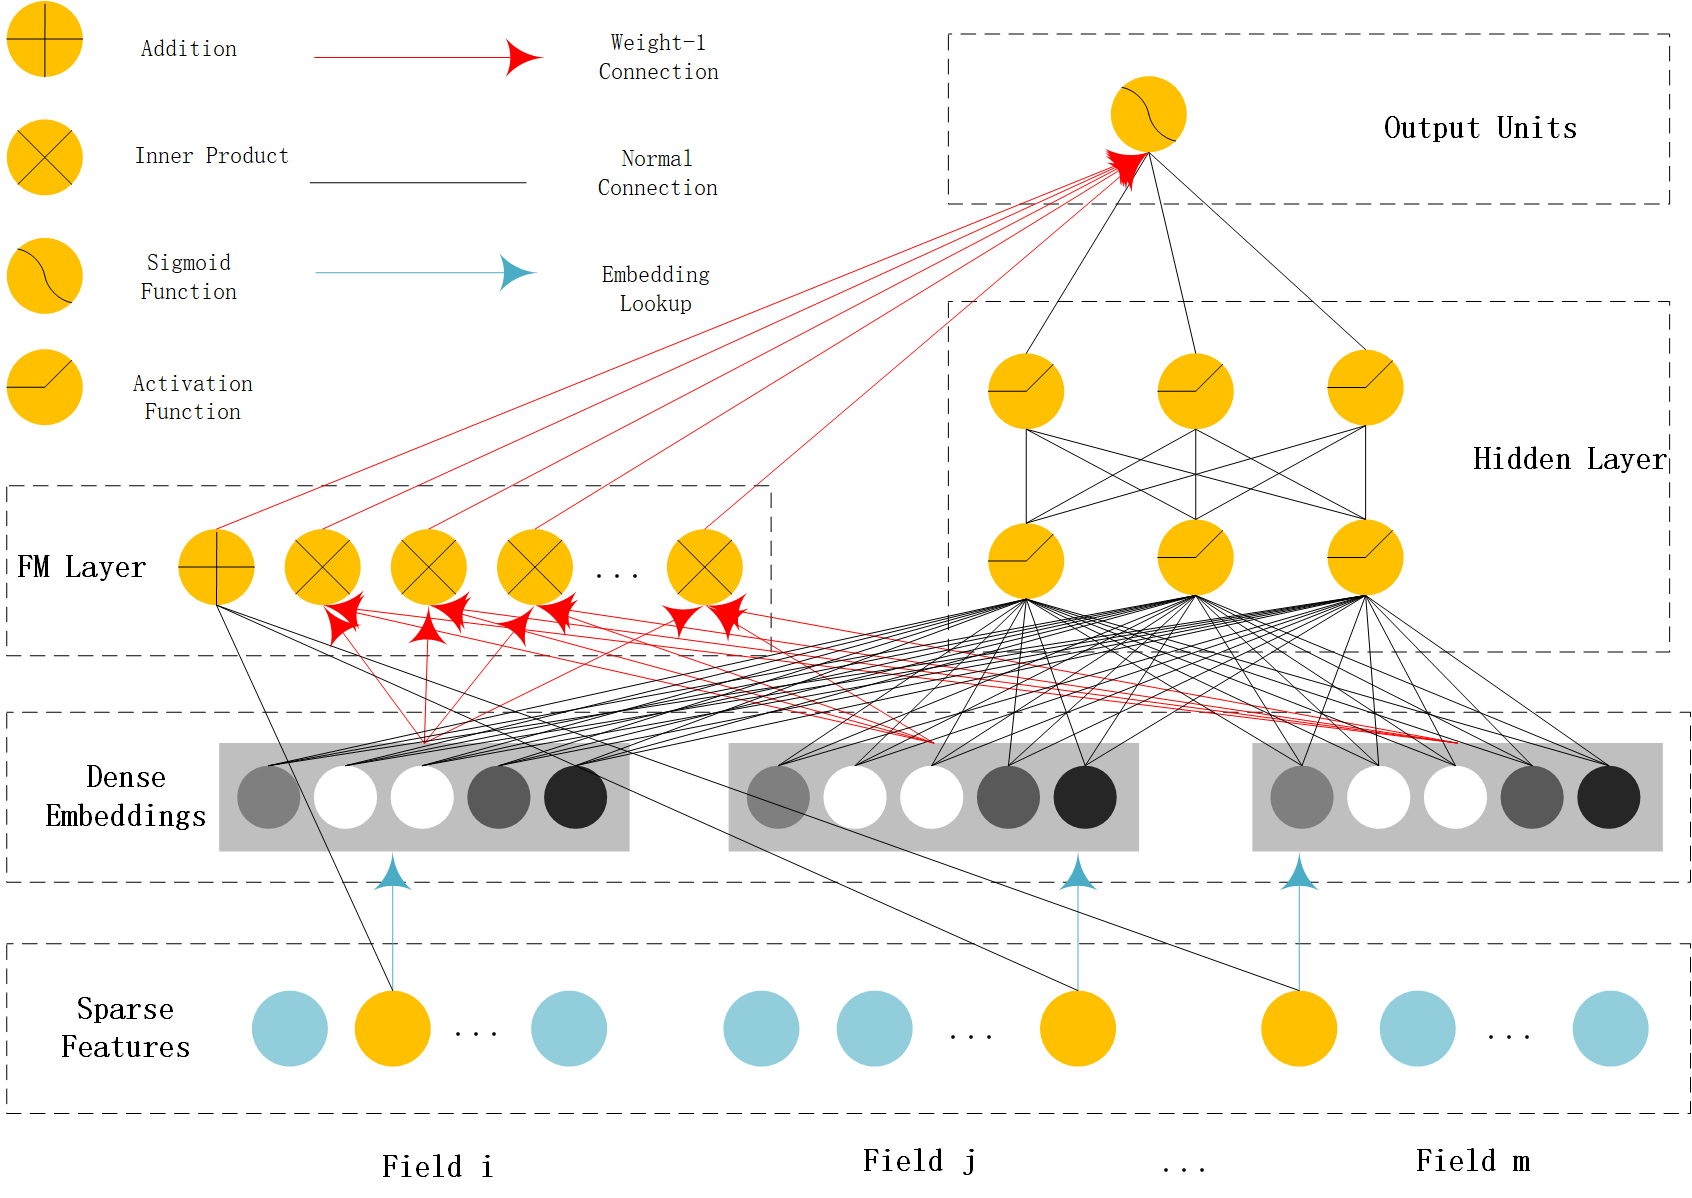
\includegraphics[width=0.95\textwidth]{images/DeepFM.png}
  \caption{DeepFM结构图\cite{DeepFM结构图}}\label{DeepFM结构图} % label 用来在文中索引
\end{figure}

可见DeepFM与Wide \& Deep的框架极为类似,差异在于在Wide部分的特征交叉输入项被替换为FM部分,FM代替Wide部分的手动特征工程构造二阶特征叉乘,从而实现了低阶的自动特征工程。DeepFM的Wide与Deep模块共享相同的由各个Field的one-hot编码横向拼接而成的高维稀疏向量输入;除此以外FM层与NN层共享相同的embedding层,从而降低了模型的复杂度,并且在embedding层训练过程中同时接受低维以及高维特征交互的反馈。在DeepFM的实验中作者对embedding层分别进行了共享与不共享的对比,发现共享效果更优。





FM部分的结构如上,FM对应的输出如下:





DNN部分的结构如下:



%%
% The BIThesis Template for Bachelor Graduation Thesis
%
% 北京理工大学毕业设计(论文)第一章节 —— 使用 XeLaTeX 编译
%
% Copyright 2020 Spencer Woo
%
% This work may be distributed and/or modified under the
% conditions of the LaTeX Project Public License, either version 1.3
% of this license or (at your option) any later version.
% The latest version of this license is in
%   http://www.latex-project.org/lppl.txt
% and version 1.3 or later is part of all distributions of LaTeX
% version 2005/12/01 or later.
%
% This work has the LPPL maintenance status `maintained'.
%
% The Current Maintainer of this work is Spencer Woo.
%
% 第一章节

\chapter{数据筛选和预处理}

\section{数据筛选}

我们的数据来自于计算机学院提供的学生数据文件,其中分为两大部分,分别是本科生信息以及研究生信息,但是其中本科生信息只包含成绩信息,而研究生信息维度较为丰富,所以使用研究生信息进行建模和推荐。其中包含2016与2017两级信息。

数据来源是教务处提供的包含学生数据的excel文件,文件共有4个,内容分别是本科生的成绩信息、研究生成绩信息、研究生学业奖学金信息以及研究生国家奖学金信息。

\subsection{本科生信息字段}

本科生成绩信息包括如下字段:

学生ID、选课课号、学年学期、课程代码、课程名称、课程性质、成绩、折算成绩、课程归属、重修标记、学分创建时间、绩点、课程属性、课程种类、考试性质、年级、学院

\subsection{研究生信息字段}

研究生成绩信息与此类似,但不同的是研究生多了一个第二课堂的excel表单,研究生与本科生信息的主要差别在于奖学金信息部分,研究生学业、国家奖学金信息均提供了8 个表单,分别是论文发表、专著论文出版、发明专利、科技获奖、科研项目、创新竞赛、荣誉称号以及其他成果,同时提供了对应每条记录的奖学金获奖情况。

研究生信息公有字段如下:

ID、学业奖学金申请等级、状态、学院培养层次、性别、民族、入学时间、学科、是否专业学位

研究生数据的论文字段如下:

论文题目、刊物会议名称、作者排序情况、论文收录情况、论文层次、中科院JCR分区大类、中科院JCR分区小类、他引情况、录用发表状态、发表时间、作者排序情况

专利字段如下:

专利名称、专利类别、专利申请号、专利申请时间、专利证书编号、专利批准日期、专利持有单位

科技获奖、创新竞赛获奖字段如下:

奖项名称、主办单位、所获奖项、获奖级别、获奖日期、奖项等级、总人数、个人排名、获奖证书编号、颁发证书单位

科研项目字段如下:

项目名称、项目类型、工作任务

出版专著字段如下:

著作名称、出版社、工作量、书号、出版日期、编著类型、作者人数、第几作者

荣誉称号/其他成果字段如下:

荣誉名称、荣誉级别、颁发单位、获得日期

在对数据进行分析之后,大致总结数据特征如下:

\section{数据库模型构建}

以数据分析为基础,这里主要对Django的数据库模式进行建构,Django是通过ORM映射对数据库进行操作,由于给定的数据源(excel文件)是关系型结构,所以我选用了关系型数据库SQLite进行数据库构建。

数据库模型构建首先需要对基础信息进行设计,基础信息按照我的构建顺序主要包括学年(期)信息、学院信息、专业信息、课程信息、学生信息。其中学年信息和学院信息是一切信息的基础,其他的信息或多或少都构建于这两个信息之上,下面对这些表中的字段与字段含义进行介绍。

\subsection{基础信息表}

\begin{enumerate}
  \item 学年(期)信息:包括学期的名称、学期起始日期、学期终止日期,通过学期信息进而转换成学年信息与数据表中的信息匹配
  \item 学院信息:主要包括学院名称
  \item 专业信息:包含专业名称、学生数量、学年ID、学年信息(大一、研一等)、学期信息以及学院信息,学年ID、学期信息以及学院信息是此表的外键,通过对学年信息进行筛选可以唯一的确定一条专业信息记录,虽然这张表可能存在一定冗余(专业名称、学生数量等)但是为了减少表之间取并的次数所以如此进行设计,未来可以将此表优化为拉链表节省存储空间加快检索速度
  \item 课程信息:包括课程名称、考核方式、课程性质、学分、课程种类、学年信息等内容,主要课程的基本信息,其中有一额外生成表为lessoninfo\_affiliatedmajor,此表生成原因是一门课程可能对应于多个学院(如高数等公共基础课),而一个学院也对应多门课程,所以产生了多对多的关系,在Django中自动将此多对多关系映射为一张额外系统表,表中内容是lesson\_info 表和affiliated\_major表的主键关联信息
  \item 学生信息:包括学生学号信息、是否为研究生、系统的登录名称、预留邮箱地址、登录密码等,学生信息与专业信息通过一额外多对多表相连,由于学生是一个实体,专业同样是一个实体,故将其之间的关系提取构建为单独关系表,在Django的代码中以through的形式表示此关系,故如下对此关系表进行解释
  \item 关系信息表:由上文可知关系信息表是通过through代码生成,Django中关系表必须包括关联的两张表的主键作为此表外键且缺一不可,所以其中包含了学生的ID(应为对应的用户ID而非学号)以及专业信息ID,并且设置了冗余学年信息避免通过专业信息查找学年信息的连接操作提升了执行速度,同时设置关系属性字段,包括研究生、本科生等不同关系类型以及学年信息,包括研究生一年级、本科生一年级等不同信息区分,并且在最后设置起始日期与终止日期字段,使此表成为一个可通过日期查询的拉链表
\end{enumerate}

如上是对基础信息表的介绍,接下来是对学生部分的个人信息表进行构造

\subsection{个人信息表}

个人信息表共包括8部分内容,其中有7个表是从所给数据文件中直接得到,分别是论文发表、专著论文出版、发明专利、科技获奖/创新竞赛、科研项目以及荣誉称号/其他成果,同时包括一个存储了学生奖学金获奖历史表,论文发表等表字段内容与excel所给字段内容一致不再赘述,值得注意的是有些空字段需要额外处理才能向数据库中录入内容,除此以外科技获奖、创新竞赛的表以及荣誉称号、其他成果表的字段内容基本一致,所以通过一个类型字段进行区分即可省略一张表,同时学生与奖学金信息同样构成了一个关系即为学生的奖学金获奖历史,这个表同样可以看作多对多关系生成的一个表,所以会额外生成一张带有学生ID和奖学金ID作为外键的表。

\subsection{奖学金表}

接下来是奖学金表的构造,因为之前考虑将系统设计为B/S架构,所以需要设计带有奖学金信息的推送网页内容,故设计奖学金信息表、奖学金信息分级表、奖学金网页内容表,这其中奖学金信息表主要包含奖学金的名称、奖励金额等,同时未来还可扩充额外要求字段。奖学金信息分类表主要是由于某个类型的奖学金可能有多个分级,需要对不同的分级进行考虑,此表能够减少冗余,并且在推送内容填充URL的时候可以直接根据奖学金是否有分级填充不同的URL提高奖学金在网页推送部分的效率,除此以外还可以增加数据库的层次化结构。同时表中的推送内容使用Markdown格式,方便如Ueditor等富文本编辑器进行编辑。同时可以使用Python 的word2md包的Markdown转换工具将word文件上传自动转为Markdown方便在线编辑使用。

\section{数据导入与数据库填充}

向数据库中填充数据使用的是Django自带的ORM映射,通过调用接口而非注入SQL命令实现更安全的数据操作方式,所有与数据填充有关的代码均在utils中,其中首先需要调用os.environ.setdefault命令读取Django启动配置,然后使用django.setup()命令实现Django的初始化,Django启动后可以通过引入不同的model对模型直接进行操作,同时还使用了python的xlrd包对excel文件进行读取。

数据库填充首先填充的是学年、学院、专业、课程以及学生信息,在填充学生个人的时候使用集合对所有数据表中的学生ID进行去重统计,除此以外还需要注意对某些特殊字段进行处理,包括对空字段进行填充等。由于在不同apps的model中设置好了部分分类字段的映射(分类字段是以CharField的形式进行保存,用元组设置了映射规则),所以需要用字典对文本进行处理与转换,最终在数据库中保存缩写后的元素。

\section{数据库信息统计与类图}

以下是对导入内容进行统计:

以下是数据库的类图:

%%
% The BIThesis Template for Bachelor Graduation Thesis
%
% 北京理工大学毕业设计(论文)第一章节 —— 使用 XeLaTeX 编译
%
% Copyright 2020 Spencer Woo
%
% This work may be distributed and/or modified under the
% conditions of the LaTeX Project Public License, either version 1.3
% of this license or (at your option) any later version.
% The latest version of this license is in
%   http://www.latex-project.org/lppl.txt
% and version 1.3 or later is part of all distributions of LaTeX
% version 2005/12/01 or later.
%
% This work has the LPPL maintenance status `maintained'.
%
% The Current Maintainer of this work is Spencer Woo.
%
% 第一章节

\chapter{特征构建与预处理}

特征的选择与构建基本上是整个推荐系统的核心所在,也是这个项目中最为复杂的部分,在项目特征的选择上,我们进行了很多的探索,接下来将一一介绍我们的工作。

\section{特征分析}

首先最简单的特征构建方法就是按照经验公式直接将学生的各项指标换算成评分来作为训练数据进行推荐,甚至于可以直接按照分数高低进行推荐,这种方法也是本科生奖学金评选经常使用的一种方法,那么在这个系统中,由于缺少对应研究生已有的经验公式,所以我没有对这部分内容进行实验,而是选择了其它方法。

对于奖学金推荐系统而言,因为推荐使用的特征是多维度的,包括论文、竞赛等诸多部分,所以我选择单独对每种类型的特征进行考虑,由于对应一个学生而言,他可能在一篇论文中有不同的作者等级,发表的论文会有不同的期刊(会议)等级,所以这些都应当作为特征构建中的评价指标,除此以外还应当考虑一个极其重要的问题即为一个学生可能有多篇论文的情况存在,而且这种现象确实已经在系统中出现,在系统中有的学生论文数量达到了3篇,更有甚者在荣誉称号一个单项上就存在7项之多,如何对其进行特征构建就成为了一个棘手的工作,如果要囊括所有学生的记录的话,那么这个特征矩阵将及其庞大,因为对应绝大部分学生来说,在某个单项(论文等)只有一项纪录,而要表示完整的单项需要的特征向量维度较高,如果只考虑竞赛一项按单人最大数量来算,那么只竞赛的表示就至少有7*n(n代表对每个记录选择的特征维数,如论文中的期刊等级以及作者排序等)个维度,所以最后我产生了两种思路,第一种思路是尽可能多的保留各单项信息,每个单项最多选取3个有价值的记录构成特征向量,或者将一个单项的所有信息累加,用公式换算为得分或者对单项信息进行无监督的聚类,将聚类标签作为特征输入推荐算法进行训练。

以上是产生的两种思路,我主要实验了第一种思路,也就是按单项最大个数对记录进行保留,但是我并没有选择简单的对特征进行筛选后直接构建特征向量,而是同时对特征使用聚类的方法以期减少特征的数量以及训练的复杂度。在这里以论文的特征向量构建为例展开分析。

以论文的特征向量构建为例,论文的特征向量主要包括论文刊载的期刊(会议)等级以及学生的作者排序,这两个数据是我们已有的,但是在给定我们的excel文件中,可以看到其他还存在一些额外的信息,比如论文期刊层次的中科院JCR分区大类、中科院JCR分区小类,以及论文他引情况等,至于为什么没有选择剩下的这3个特征进行构建,是因为对于绝大部分论文而言,前两个特征已经足够进行评级并且剩下的3个特征存在的问题分别是JCR分区大类和分区小类没有包括部分国际期刊的分类而完全归于其他分区,导致对部分国际、国内和部分国际、国内会议的区分不够明确,他引情况的问题是他引情况可能随时间变化较大,如较早发表的论文的引用数量较多,而较晚发表的论文可能引用数量不足或根本为0,同时如何获取论文引用数量也是一个很困难的现实,因为我一开始曾经考虑对知网信息进行爬取获得论文的关键词、摘要等按照中文NLP方法以及one-hot编码对论文内容进行简单分类,但是一方面知网有完整的反爬机制除此以外对知网内容进行爬取可能会导致学校IP被暂时封禁,所以最终放弃了这种想法。但是我们选择了使用聚类的方法对论文数据进行处理,接下来将对聚类的实现展开介绍。 

\section{聚类方法}

\subsection{PCA/TSNE成分分析}

聚类使用的主要方法均为无监督聚类,以典型的KMeans方法为例,我们首先对论文数据进行了清洗,并且保留了聚类所用到的两个特征--论文作者排序以及期刊(会议)等级,并且使用TSNE以及PCA两种方法对数据进行了主成分分析以及可视化处理,同时我们使用了one-hot encoding以及label encoding两种方法将文字特征转化为数值特征,理论上而言期刊(会议)等级和作者排序均存在大小关系,所以我们构建的label encoding也是以高等级期刊、高作者排序对应数值低而进行,因此我们自主设定了排序等级,以期刊(会议)等级的label encoding为例:

由上可知期刊(会议)等级排序共8类,所以我们对其进行了一一映射,同时也可以对其进行one-hot encoding,对one-hot encoding后的样本进行TSNE可视化以及主成分分析后的结果如下:



可见主成分在6~8左右(one-hot后的特征向量)对原始特征的还原度较好,在这里可以选择对主成分进行提取;而TSNE的可视化结果则显示样本呈现某种特殊的分布规律,初步验证数据呈现规律分布可以进行聚类。

\subsection{K-Means 聚类}

接下来我首先进行的是使用KMeans方法聚类,根据KMeans的官方文档,对类别特征最好进行one-hot encoding后去除自身的欧几里得距离特征进行聚类更为合适,虽然KMeans对噪声敏感而且初始点的选择可能会影响聚类效果,但KMeans作为一种容易理解简单易懂而且执行速度较快的聚类算法在这种小量数据集上可以有较好的表现,所以我首先选择了KMeans对其进行聚类。由于KMeans要手动选取聚类类数k,所以我首先进行了k=5的聚类,效果虽然不太理想但是证明了KMeans在这个数据集是有效的,接着我对KMeans的聚类结果进行了可视化展示,分别展示了聚类不同类中数据个数以及PCA主成分分析后提取的主成分分布图,结果如下:



以上左图展示了聚类个数以及聚类的标签之间的关系,右图是PCA的主成分分布情况,从图中来看label中有一个类的数量极多,这个类根据后续的查询也是所有论文中最多的两个成分组成的类,分别是第一作者以及国际会议。

接着我对KMeans进行了优化,主要的优化为以不同的k值进行实验并评价聚类效果,对于聚类效果的评价,我选用的是轮廓系数(silhouette score)和Calinski-Harabasz系数。轮廓系数取值在[-1,1]之间,接近0表示重叠的群集,负值通常表示样本分配给错误的聚类,轮廓系数的值大表示同类样本相距近,不同样本相距远,聚类效果较好;c-h系数主要作用是计算同一类别内部的协方差大小衡量类内的相似性,类内数据的协方差越小越好,类间的协方差越大越好,对于C-H系数而言C-H系数值越高说明聚类的区分度越高。那么我通过这两个指标可视化输出不同k值的系数变化曲线来确定k的最优值。结果如下:



可以看到k=7左右的聚类效果较好,那么在这样的情况下我们考虑使用其它方法进行聚类并评价聚类效果选择最优算法进行聚类,选择的其他算法包括谱聚类以及HDBSCAN。

\subsection{HDBSCAN 聚类}

为了实现自动化的聚类个数n选择,我使用了HDBSCAN进行实验,在HDBSCAN的可视化工作上我生成了HDBSCAN的集群层次结构、生成的提取簇以及压缩聚类树,聚类的效果如下:



可以看到虽然HDBSCAN的效果不甚理想,主要原因是由于HDBSCAN本身是对平面上的数据进行分类,对于大量数据重合的情况分类效果尤其是提取簇和压缩树的效果不明显,但是HDBSCAN也将聚类簇数设置为6,如果再加上label为-1的列(对于HDBSCAN不属于任何聚类簇的标签)那么簇数为7,与KMeans的效果相同,再一次印证了k=7是较优结果。

\subsection{谱聚类}

除此以外我们也使用了谱聚类对聚类结果进行测试,谱聚类同样使用了轮廓系数以及Calinski-Harabasz系数对不同的聚类簇数进行测试,同时也对gamma值进行了调参,gamma是谱聚类算法核函数参数,可视化输出效果如下:



同样可以看到在7-1的组合左右谱聚类的轮廓系数达到最优,但是值得注意的是C-H系数呈现下降的态势,但是总体而言最终还是选择k=7,gamma=1进行聚类较为合适。

\section{特征构建总结}

其他的方法包括单独构建特征,不通过聚类的方法对特征进行one-hot encoding或label encoding直接作为数据特征进行训练或者将聚类结果作为特征而删除所有单独特征节省特征矩阵的长度,但是以上方法由于时间原因未能尝试,尤其是将聚类结果作为全部特征的特征构建也不失为一个构建模型好的选择,这样的方法更适合与对推荐模型进行融合。

除此以外可以考虑的方法还有对连续特征离散化,比如将成绩将成绩分段统计作为特征进行训练。这样可以避免连续取值需要归一化的问题,并且可以更清晰的对分数分布等特征在模型中的作用进行统计。

\section{csv生成}

在生成csv的过程中我们也充分考虑了论文等级论文期刊存在的偏序关系,以论文的排序举例,首先是按照用户的user\_id进行排序,接下来按照论文层次进行排序,然后按照论文的作者等级进行排序,最后按照论文的期刊等级排序,在这样的排序条件下,虽然可能出现一个人有多个论文的情况,但是可以保证所有的数据都是以特定规则排列而不是无规则排列,这样在模型训练过程中会更为准确。除此以外对于论文等特征我们也统计了论文数量作为特征之一,而且在实验中证明论文数量也是影响奖学金评定的重要因素。

在特征设计的过程中为了将one-hot后离散的稀疏特征进行降维可以选择多种方法,其中比较典型的方法为借用word2Vec的思想加入embedding层进行嵌入训练将特征转化为低维稠密且元素不为0的特征,或者通过决策树等方式对特征进行降维处理。我们在DeepFM中验证了前一种方法,并且使用了XGBoost验证了第二种方法。

% 这里插入一个参考文献,仅作参考

\subsection{三级题目}

\textcolor{blue}{正文部分:宋体、小四;正文行距:22磅;间距段前段后均为0行。阅后删除此段。}

\textcolor{blue}{图、表居中,图注标在图下方,表头标在表上方,宋体、五号、居中,1.25倍行距,间距段前段后均为0行,图表与上下文之间各空一行。阅后删除此段。}

\textcolor{blue}{\underline{\underline{图-示例:(阅后删除此段)}}}

\begin{figure}[htbp]
  \vspace{13pt} % 调整图片与上文的垂直距离
  \centering
  
\includegraphics[]{images/bit_logo.png}
  \caption{标题序号}\label{标题序号} % label 用来在文中索引
\end{figure}

\textcolor{blue}{\underline{\underline{表-示例:(阅后删除此段)}}}

\begin{table}[htbp]
  \linespread{1.5}
  \zihao{5}
  \centering
  \caption{统计表}\label{统计表}
  \begin{tabular}{*{5}{>{\centering\arraybackslash}p{2cm}}}
    \hline
    项目    & 产量    & 销量    & 产值   & 比重    \\ \hline
    手机    & 1000  & 10000 & 500  & 50\%  \\
    计算机   & 5500  & 5000  & 220  & 22\%  \\
    笔记本电脑 & 1100  & 1000  & 280  & 28\%  \\ \hline
    合计    & 17600 & 16000 & 1000 & 100\% \\ \hline
    \end{tabular}
\end{table}

\textcolor{blue}{公式标注应于该公式所在行的最右侧。对于较长的公式只可在符号处(+、-、*、/、$\leqslant$ $\geqslant$ 等)转行。在文中引用公式时,在标号前加“式”,如式(1-2)。阅后删除此
段。}

\textcolor{blue}{公式-示例:(阅后删除此段)}
% 公式上下不要空行,置于同一个段落下即可,否则上下距离会出现高度不一致的问题
\begin{equation}
    LRI=1\ ∕\ \sqrt{1+{\left(\frac{{\mu }_{R}}{{\mu }_{s}}\right)}^{2}{\left(\frac{{\delta }_{R}}{{\delta }_{s}}\right)}^{2}}
\end{equation}

%%
% The BIThesis Template for Bachelor Graduation Thesis
%
% 北京理工大学毕业设计(论文)第一章节 —— 使用 XeLaTeX 编译
%
% Copyright 2020 Spencer Woo
%
% This work may be distributed and/or modified under the
% conditions of the LaTeX Project Public License, either version 1.3
% of this license or (at your option) any later version.
% The latest version of this license is in
%   http://www.latex-project.org/lppl.txt
% and version 1.3 or later is part of all distributions of LaTeX
% version 2005/12/01 or later.
%
% This work has the LPPL maintenance status `maintained'.
%
% The Current Maintainer of this work is Spencer Woo.
%
% 第一章节

\chapter{实验过程}

\section{XGBoost}

XGBoost是一种常用的提升树模型算法,它在推荐系统和分类问题中有着优异的效果,XGBoost基于GBDT(梯度提升决策树)实现,它和GBDT相同都是Boosting算法一种,Boosting算法的思想是将许多弱分类器如CART回归树模型等集成在一起,形成一个强分类器。

\subsection{训练集、测试集与验证集划分}

在我们的系统中,首先使用了XGBoost单独进行分类并查看分类的准确率、auc等评价指标,并且将此作为baseline,同时我们使用Hyperopt对XGBoost进行自动化调参,在XGBoost的实验过程中,我们首先对数据集进行了划分,使用常见的经验公式对数据集进行了8-2划分,划分后的训练集共100条数据,测试集共26条数据。

接下来就是对XGBoost进行建模,XGBoost使用xgboost包实现调用,在调用XGBoost的过程中,我们使用了K-fold的方法进行了5折交叉,通过调用XGBoost自带的cv函数实现比sklearn中kfold split更快的交叉运算。在将训练集和测试集输入XGBoost之前,首先通过xgb自带的DMatrix格式转化为XGBoost自有格式并且进行了填空处理,这样的优点是运算速度更快。

\subsection{Hyperopt自动化调参}

然后我们通过引入hyperopt定义目标函数,hyperopt是一个基于Python实现的Sklearn超参数优化类库,一般而言使用hyperopt有四个主要部分,分别是定义最小化/最大化的目标函数作为优化目标;其次是定义搜索空间,也就是超参数的;接下来定义存储搜索过程中所有点组合以及效果的方法;最后要确定在搜索过程中要使用的搜索算法。

我们在实验过程中对XGBoost选择的目标函数有两种,分别是验证集的mlogloss以及auc值,对于mlogloss而言,我们需要对其进行最小化,而auc则是进行最大化搜索;定义的参数搜索空间如\ref{hyperopt-param-space}所示:
\begin{figure}[htb]
  \vspace{13pt} % 调整图片与上文的垂直距离
  \centering
  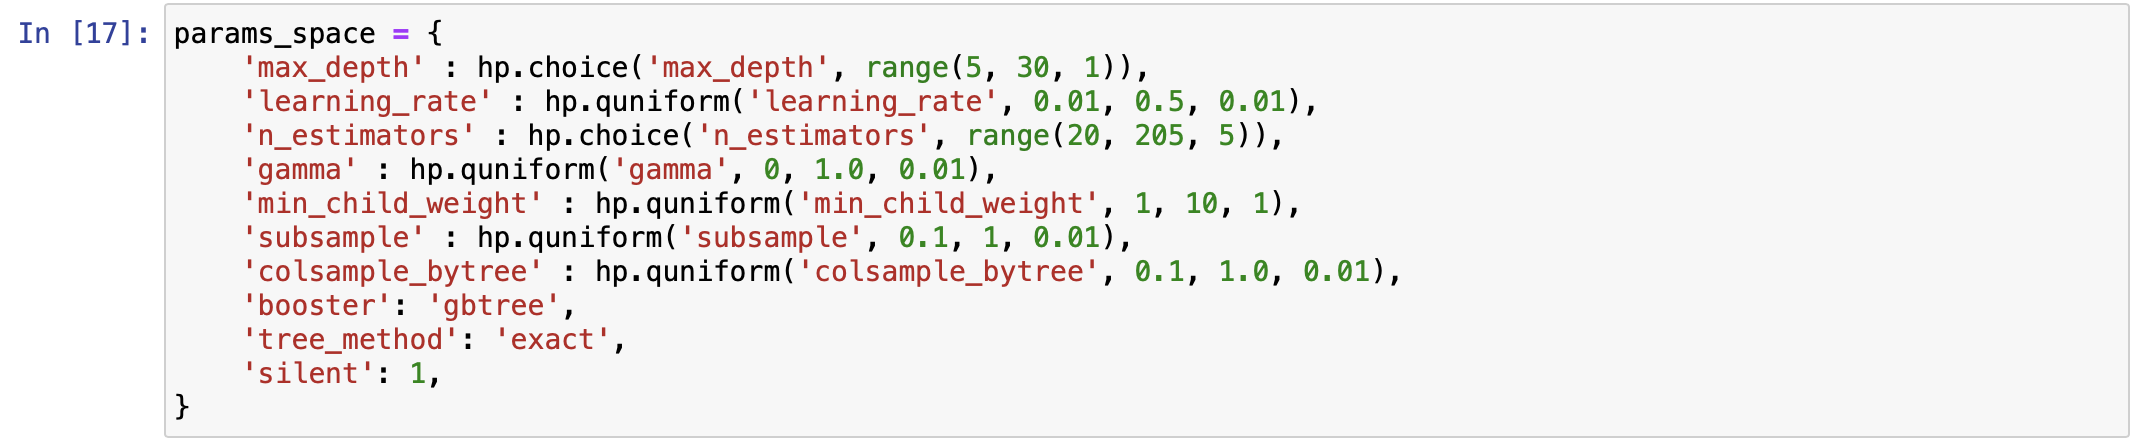
\includegraphics[width=0.95\textwidth]{images/XGBoost-hyperopt-param-space.png}
  \caption{hyperopt参数空间}\label{hyperopt-param-space} % label 用来在文中索引
\end{figure}

\newpage
其中max\_depth是决策树的最大深度,在这里搜索空间从5到30以1递增,
learning\_rate是学习率,学习率从0.01到0.5以0.01递增,
n\_estimators是决策树的数量,
gamma是控制后剪枝的参数,
min\_child\_weight是控制孩子节点当中最小的节点的样本权重和,如果叶子节点的样本权重和小于min\_child\_weight则对叶子节点拆分结束,在现行的回归模型中,这个参数的主要作用是控制过拟合,它代表了建立模型需要的最小样本数;
subsample同样是用于控制模型过拟合的一个参数,它的含义是用于训练模型的子样本在总样本中的比例;
colsample\_bytree是在建立决策树时对特征随机采样的比例;
booster使用的是gbtree,也就是树模型;
tree\_method表示计算时使用的树方法,这里选择的是准确的计算值,同样可以使用近似计算来加快运算速度。

在定义搜索空间后定义目标函数,这里的目标函数代码如\ref{hyperopt-objective-function}所示:
\begin{figure}[htb]
  \vspace{13pt} % 调整图片与上文的垂直距离
  \centering
  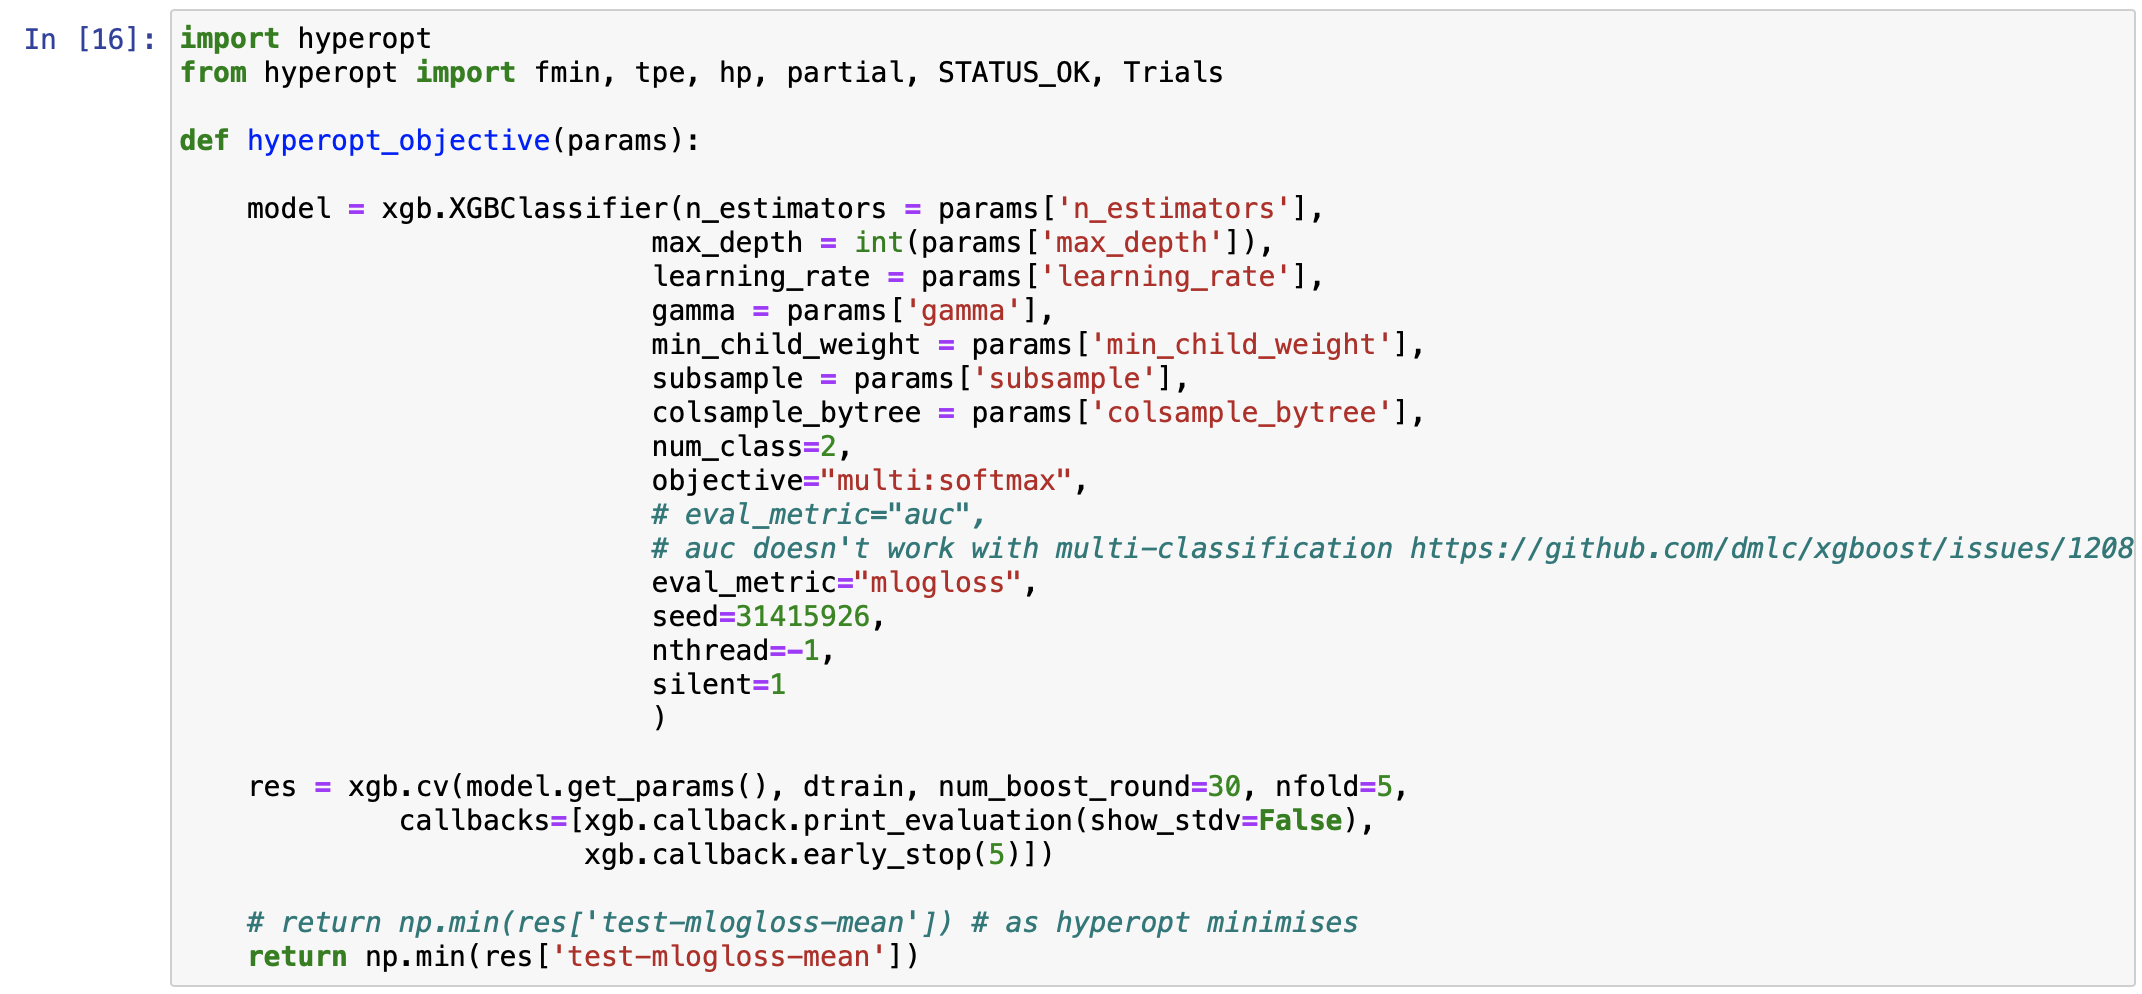
\includegraphics[width=0.95\textwidth]{images/XGBoost-hyperopt-objective-function.png}
  \caption{hyperopt目标函数}\label{hyperopt-objective-function} % label 用来在文中索引
\end{figure}

可以看到这里使用的是test-mlogloss-mean作为优化函数进行优化,每次选择test-mlogloss-mean的最小值返回给hyperopt进行效果验证,它的返回值来自于xgboost的k-fold方法,同时为了防止过拟合的现象使用了early\_stopping方法在验证集验证,使用的验证函数同样是mlogloss

同时在这里需要特别注意的一点在于XGB是无法使用auc作为eval\_metric,在XGBoost的issue中可以看到auc目前不支持在XGB上使用。

除此以外对于XGBoost模型分别在两种不同编码格式的数据集上进行了测试,首先我们在one-hot encoding的数据集上进行了测试。

\subsection{数据编码方式效果对比}

根据XGBoost模型的文档,它推荐我将所有的类别特征转化为独热编码,XGBoost对于特征的值仅接受数字类型的特征,因此必须进行独热编码。 但是如果有类似的数字特征变量并且对类别使用数字占位符(例如,{男,女,未知}分别为{1,2,3}),则对于XGBoost的学习而言这些特征是不能正确表示的,因为这些特征是存在偏序关系的,而原始类别没有与之关联的任何固有顺序,但是XGBoost模型可能会错误的学习数值带有的偏序关系而导致误差。

所以我们考虑将论文的作者顺序等通过one-hot encoding转化为独热编码后输入XGBoost,虽然也有人指出one-hot encoding可以将距离计算变得更为合理,但对于离散特征而言,不需要使用one-hot encoding即可较好的进行距离计算,对于某些基于树的算法而言,变量的处理并不是基于向量空间而只是作为类别符号,其不存在偏序关系故而不需要进行one-hot encoding。而独热编码反而增加了决策树的深度。

hyperopt的默认搜索算法是tpe,这是一种类似于遗传算法的搜索算法,它是一种启发式的最优化方法。

首先将one-hot encoding后的特征输入XGBoost中通过hyperopt自动化调参,数据集共有118维特征,学习目标为多分类(multi:softmax),验证集使用目标函数为mlogloss,测试后的最优参数下测试集的loss为0.41,而在此情况下训练集的loss为0.21,可以看到XGBoost对于训练集出现了一定程度的过拟合情况。同时在这种情况下gamma值为0.84,学习率为0.45,树的最大深度为12,subsample取值为1,这里是值得注意的,因为subsample为控制过拟合的参数,它使用全部训练集输入对XGBoost的树模型进行训练在一定程度上也导致了测试集的loss较差,特征随机采样比例为0.79,叶子节点的最小权重和为2,决策树个数为14。

使用最优参数对XGBoost模型进行训练,得到的CrossValMean为0.78,准确率为0.61,可以看到这个结果不甚理想,同时特征重要性结果如图\ref{XGBoost-one-hot-feature-importance}所示:
\begin{figure}[htb]
  \vspace{13pt} % 调整图片与上文的垂直距离
  \centering
  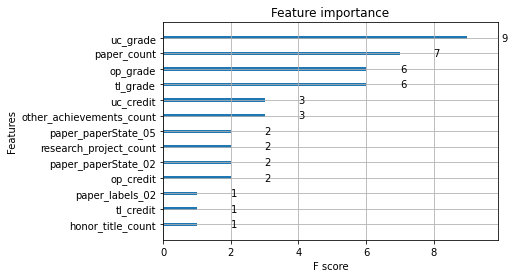
\includegraphics[width=0.95\textwidth]{images/XGBoost-one-hot-feature-importance.png}
  \caption{XGBoost one-hot 特征重要性}\label{XGBoost-one-hot-feature-importance} % label 用来在文中索引
\end{figure}

可以看到其中最为重要的特征是未分类课的成绩,其次是发表论文的数量,然后是选修课成绩、总加权平均成绩以及未分类课学分,然后是其他类型奖励的数量、以及论文的层次等。综上可以看到在整个过程中对模型影响较大的因素为成绩因素和论文质量。

\begin{figure}[htb]
  \vspace{13pt} % 调整图片与上文的垂直距离
  \centering
  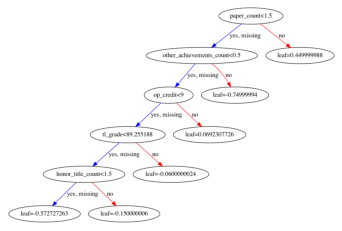
\includegraphics[width=0.5\textwidth]{images/XGBoost-one-hot-decision-tree.png}
  \caption{XGBoost one-hot 生成树(其一)}\label{XGBoost-one-hot-decision-tree} % label 用来在文中索引
\end{figure}
图\ref{XGBoost-one-hot-decision-tree}是其中一棵生成树的图片,可以看到树的深度为6,首先分裂的节点是论文数量。

接下来我们又对使用Label Encoding的编码数据集进行了测试,测试的结果大大出乎了我们的意料,在hyperopt优化参数不变的情况下,Label Encoding的效果远好于One-hot编码后的效果,虽然XGBoost的文档推荐使用One-hot编码,而且原理上One-hot不影响决策树的效果,但是实际上XGBoost在小量数据上对大量特征的分裂决策效果依然不是很好。

Label Encoding的数据集中特征向量的维数为61,经过测试XGBoost在Label Encoding数据集上的最优参数为特征随机采样比例0.45,gamma为0.99,学习率为0.17,最大深度为23,最小叶子节点权重和为2.0,决策树个数为26,决策树模型训练样本比例subsample=0.7,在最优参数下进行模型训练得到的FinalCrossMean为0.79,虽然和使用One-hot encoding的结果相差不大,但是实际上模型在测试集的准确率提升到了96\%,远高于独热编码后的结果,特征重要性排序如图\ref{XGBoost-label-encoding-feature-importance}所示:
\begin{figure}[htb]
  \vspace{13pt} % 调整图片与上文的垂直距离
  \centering
  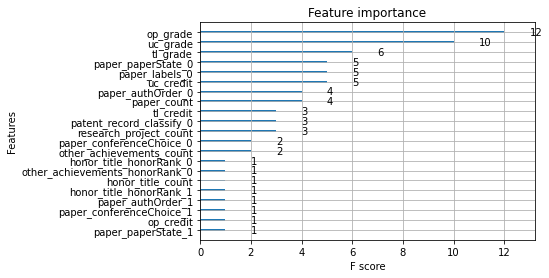
\includegraphics[width=0.95\textwidth]{images/XGBoost-label-encoding-feature-importance.png}
  \caption{XGBoost label-encoding 特征重要性}\label{XGBoost-label-encoding-feature-importance} % label 用来在文中索引
\end{figure}


可以看到参与训练的特征数量明显变多,虽然成绩特征依然重要,但是最重要的特征从未分类加权平均成绩变为选修课加权平均成绩,总成绩的重要性基本不变,接下来第一篇论文的论文层次和论文聚类的标签也对结果有重要作用,除此以外第一篇论文的作者排序以及发表论文的总数量等起次等作用。未分类课的学分以及总学分在特征重要性中也有一定比重。但是对于使用独热编码的特征,专利、研究项目等很多特征并没有考虑在内。而在 Label-Encoding 方法下,专利和研究项目的数量、其他成果的数量、荣誉等级和荣誉数量等都在模型决策树构建中发挥作用,除此以外模型对第二篇论文的情况也纳入了考虑范围,包括第二篇论文的作者顺序、期刊等级以及论文层次等。

所以综上可以看出One-hot encoding的模型相比于Label encoding的模型效果相差甚远,可能原因是One-hot的特征矩阵较为稀疏,模型的迭代次数不足,而且模型在自动化调参过程中subsample比例过高导致模型出现了比较严重的过拟合问题,以上都是未来可以进行实验和改进的方向。Label encoding的XGBoost的一棵生成树如图\ref{XGBoost-label-encoding-decision-tree}所示。
\begin{figure}[htb]
  \vspace{13pt} % 调整图片与上文的垂直距离
  \centering
  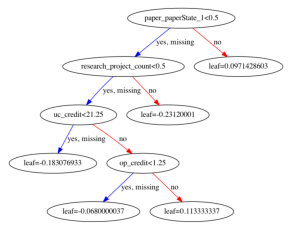
\includegraphics[width=0.6\textwidth]{images/XGBoost-label-encoding-decision-tree.png}
  \caption{XGBoost label-encoding 生成树}\label{XGBoost-label-encoding-decision-tree} % label 用来在文中索引
\end{figure}

在构建XGBoost单独进行预测后,我们也考虑将XGBoost的决策树输出作为新的特征与其他简单模型融合,可以考虑使用XGBoost+贝叶斯或者XGBoost+LR逻辑回归等。

\section{XGBoost与逻辑回归融合}

我们同样进行了对比实验,以上述表现效果较好的Label-Encoding XGBoost模型作为新特征的全部或者一部分分别进行实验。

首先是对XGBoost决策树的特征进行构建,特征构建的原理是由于XGBoost的决策树存在多个输出,对于一条数据而言它的权值会由不同的叶子节点输出,所以将所有的叶子节点视为0-1编码的one-hot 向量,即可构建一个长度=叶子节点总数的特征向量。

对叶子节点输出进行获取的方法是XGB自带的apply方法,apply的结果是决策树对应的叶子节点值,若没有叶子节点(max\_length = 1),那么此值为0,否则>=1的整数,所以先去除没有叶子节点的决策树,通过自定义的get\_cols\_del函数获取apply后形成的DataFrame中需要删除的列标号,然后用del\_cols函数删除DataFrame中对应的无信息的列(全0),再通过one-hot encoding的形式自定义一个One-hot Label Encoder进行one-hot编码后得到对应的稀疏特征矩阵,这样可以在一定程度上压缩特征空间的大小,并且能够提取高维的特征交互信息,然后将此结果输入一个简单的线性分类模型中,同时还可以省去归一化的步骤。

将构建好的特征输入到一个简单的逻辑回归分类器当中,此时输出经过one-hot encoding后的特征共98维,略微少于完全使用one-hot的118维,在使用默认参数进行训练后对测试集进行了准确率测试,测试结果与XGBoost相同但是auc值高于单独使用XGBoost结果0.25,此时auc值为0.97,虽然提升效果不明显但是在全数据集上进行准确率测试发现准确率从0.89提升到0.97,auc从0.83提升到0.963,所以逻辑回归和XGBoost决策树节点输出结果结合比较好的解决了模型的拟合问题,并且进一步提升了模型的准确率。

除此以外我们还使用XGBoost决策树节点输出结果与原有特征进行融合,以此构建一个既包含高维特征交叉也包含低维特征的特征向量。同样将80\%的数据用于训练20\%数据用于测试,在这种情况下模型出现了一定的过拟合情况,对测试集的准确率下降到92\%,auc下降到93\%,但全数据集的准确率提升到98\%,auc提升到98.7\%,虽然提升不明显,但是无论在accuracy或者auc上均有提升,所以可以看出融合了原有低维特征和XGBoost输出高维特征的特征向量还是使结果呈现了一定的上升趋势。

\section{XGBoost与贝叶斯分类器融合}

那么顺着这个思路我们又进行了一系列的实验,包括将逻辑回归模型替换为Bayes分类器或SVM等并分别对它们的表现进行测试,结果如下:


\begin{table}[htbp]
  \linespread{1.5}
  \zihao{5}
  \centering
  \caption{贝叶斯分类器效果比较}\label{贝叶斯分类器效果比较}
  \begin{tabular}{*{5}{>{\centering\arraybackslash}p{2cm}}}
    \hline
        & Test-Accuracy    & Test-AUC    & Train-Accuracy   & Train-AUC    \\ \hline
    Pure BernoulliNB    & 0.884  & 0.888 & 0.72  & 0.704  \\
    BernoulliNB + XGBoost   & 0.923  & 0.918  & 0.83  & 0.792  \\
    GaussianNB + XGBoost & 0.885  & 0.906  & 0.82  & 0.862  \\ 
    MultinomialNB + XGBoost  & 0.923 & 0.918 & 0.81 & 0.818 \\ \hline
    \end{tabular}
\end{table}

\newpage
可以看到不同分布函数的贝叶斯分类器的效果不同,其中效果最好的是高斯分布的贝叶斯,这种情况出现可能和成绩、竞赛等分布符合高斯分布有关。 可以看到多项式贝叶斯模型在测试集的效果最好,但是从训练集的准确度和auc值看,可能存在欠拟合的问题,并且在整个数据集上进行测试后可以发现它整体的效果不如高斯分布贝叶斯。伯努利分布的贝叶斯与多项式贝叶斯一样在测试集上效果好但是在训练集上效果一般,同样可以考虑测试集和训练集划分的问题。单独使用贝叶斯对不包含XGB输出的效果是最差的,说明Bayes没有对高维和低维特征的融合进行较好的处理。

同时我们还使用了GBDT、SVM等作为对特征融合的向量的输入模型。其中GBDT+XGBoost的效果最好,这是由于GBDT与XGBoost一样都是树模型,但是没有使用GBDT的原因是GBDT的模型较为复杂,不利于降低模型复杂度,而且训练比逻辑回归要困难得多。



\section{神经网络模型}

% \subsection{DeepFM}

关于神经网络模型,我们使用了DeepFM,通过FM进行自动特征交叉,并验证了算法的效果。

首先对DeepFM中的DenseFeature 与 SparseFeature进行处理,DeepFM中的DenseFeature指数值类特征或类似连续或带有特定偏序关系的特征,SparseFeature一般为CategoricalFeature或类似离散数值特征。通过函数SparseFeat实现稀疏特征矩阵构造,其中DeepFM使用默认参数进行实验(
dnn\_hidden\_units=(128, 128), l2\_reg\_linear=1e-05, l2\_reg\_embedding=1e-05, l2\_reg\_dnn=0, seed=1024, dnn\_dropout=0, dnn\_activation='relu', dnn\_use\_bn=False, task='binary'),其使用的embedding层的size为4。

以0.5为界对DeepFM的输出进行处理,则在使用相同数据集划分(测试集-训练集)种子情况下DeepFM在测试集上准确率为0.92,略低于使用label-encoding的 XGboost,在整个训练集上的准确率是0.82,整体为0.84左右,与单独使用 XGBoost 相比存在一定差距。但是相比使用 one-hot encoding 的 XGB 模型进步明显。


% \begin{figure}[htbp]
%   \vspace{13pt} % 调整图片与上文的垂直距离
%   \centering
%   
\includegraphics[]{images/bit_logo.png}
%   \caption{标题序号}\label{标题序号} % label 用来在文中索引
% \end{figure}

% \textcolor{blue}{公式标注应于该公式所在行的最右侧。对于较长的公式只可在符号处(+、-、*、/、$\leqslant$ $\geqslant$ 等)转行。在文中引用公式时,在标号前加“式”,如式(1-2)。阅后删除此
% 段。}

% \textcolor{blue}{公式-示例:(阅后删除此段)}
% % 公式上下不要空行,置于同一个段落下即可,否则上下距离会出现高度不一致的问题
% \begin{equation}
%     LRI=1\ ∕\ \sqrt{1+{\left(\frac{{\mu }_{R}}{{\mu }_{s}}\right)}^{2}{\left(\frac{{\delta }_{R}}{{\delta }_{s}}\right)}^{2}}
% \end{equation}


% 结论:在结论相应的 TeX 文件处进行结论部分的撰写
%%
% The BIThesis Template for Bachelor Graduation Thesis
%
% 北京理工大学毕业设计(论文)结论 —— 使用 XeLaTeX 编译
%
% Copyright 2020 Spencer Woo
%
% This work may be distributed and/or modified under the
% conditions of the LaTeX Project Public License, either version 1.3
% of this license or (at your option) any later version.
% The latest version of this license is in
%   http://www.latex-project.org/lppl.txt
% and version 1.3 or later is part of all distributions of LaTeX
% version 2005/12/01 or later.
%
% This work has the LPPL maintenance status `maintained'.
%
% The Current Maintainer of this work is Spencer Woo.
%
% Compile with: xelatex -> biber -> xelatex -> xelatex

\unnumchapter{结~~~~论}
\renewcommand{\thechapter}{结论}

\ctexset{
  section/number = \arabic{section}
}

% 结论部分尽量不使用 \subsection 二级标题,只使用 \section 一级标题

% 这里插入一个参考文献,仅作参考
通过这个毕业设计,我基本上完整的进行了数据预处理、数据仓储、特征构建、特征工程、算法选择与比较以及预测推荐的完整流程。虽然整个系统在训练当中的数据量偏少,特征维数较少而且很多功能都还没有实现,但是整体而言这让我体会到了一个完整的数据挖掘的流程,使我获益匪浅。

\section{特征构建与特征工程}

值得注意的是在挖掘过程中,XGBoost使用one-hot 编码以及label encoding 两种编码方式的结果有明显差异,再一次提示我在进行特征构建时要注意考虑特征是否存在偏序关系。如果只是简单的类别特征,如国家等,可以考虑使用one-hot encoding 的方法进行编码,否则最好考虑两种方法融合或者进行比较。

除此以外特征构建过程中我们没有使用特征重要性或者PCA主成分分析等方法对特征进行降维,而是使用了聚类的方法以期可以对特征降维。从结果来看聚类的标签在模型权重的重要性比重不大,可能是由于数据量较少导致模型训练过程中没有使用到全部的特征,这一点在XGB 模型的特征重要性当中有比较明显的体现,为了日后系统扩展的需求,暂时先不对特征进行筛选或主成分分析来降维。

在特征构建的过程中我们也没有使用手工特征交叉,主要原因是对于数据的理解不够深入,不知道怎么进行特征交叉的效果比较好。而且整体来看最后的特征哪怕是label encoding的结果也有超过60维,而且很多特征在训练中起到的作用很小,甚至对模型是负优化,可以考虑在未来剔除这些特征,如专利的分类(发明专利/其他)等。在特征构建的过程中只使用了两类具有代表性或数量较多的标签作为label进行训练,未来也可以加入国奖等其他奖学金将XGBoost模型修改为多分类,多分类下可以将一类作为正类其他类作为负类计算某条数据的概率并以阈值为过滤条件进行推荐,这样可以实现Top-N推荐的功能。

同时在多分类下也可以对网络输出层进行修改,使神经元个数与分类标签个数相等,从而构建一多分类器。也可以加入Sigmoid进行分类器构建。

\section{模型训练与融合}

在这一部分中我们分别进行了单独的XGBoost分类器构建、朴素贝叶斯分类器构建以及SVM模型构建等多种模型,结果上XGBoost无论在训练精度或者AUC值上都占有明显优势。体现了XGBoost在处理这种少量有关联特征的数据时的优秀效果,

在XGBoost的特征构建过程中,可以看做我们对模型进行了融合,将XGBoost的结果与逻辑回归分类器进行融合。但是这里的缺点是最后形成的模型并不是一个端到端的模型,而是需要先对 XGB 进行训练,并没有达到联合训练的效果。所以这种方法整体的训练难度较高,但是值得肯定的是这种方法的收益率是很明显的,XGBoost的apply方法的叶子节点输出可以看作是高维的特征交叉结果,而对低维特征的保留与逻辑回归方法的运用则可以看作是另一种Wide \& Deep模型的实现思路,不同的是Wide \& Deep 还使用了embedding层进行了降维,而我们没有对特征进行embedding处理。
下一步可以考虑将XGBoost的apply输出当作Wide \& Deep中Wide部分的输入,代替手动特征工程的结果对网络进行训练。

但是无论如何XGBoost和神经网络相比它的优势是很明显的,具体体现在XGBoost的模型训练速度更快、精度更高。而且可以很方便的将XGBoost的结果与其他模型融合。也进一步验证了对于中、少量的结构化数据XGBoost的效果一般比神经网络更优。

可以考虑使用融合模型的方法训练,但是没有采用这种方法的原因是单纯的XGBoost效果很好,采用这种方法融合意义不大。

同时还应当注意XGBoost在训练过程中的特征重要性,可以看到论文数量以及成绩两因素对得奖结果的影响是非常明显的,从特征上可以看出学分以及对应的单项平均成绩在使用两种不同编码方法的XGBoost模型中所占权重都比较大,其次在使用label-encoding的XGB模型中它学习到了更多特征相关性,值得注意的是未分类课成绩、选修课成绩、加权平均成绩在两模型中所占比重都比较高,第一篇论文在模型中所占权重较高,而且使用label encoding的模型在使用论文特征、其他成果特征、荣誉获奖特征、科研项目特征之外还学习到了专利这个大类。但是两个模型都没有学习到竞赛这个大类的特征,可能是数据量较少或竞赛大类缺少竞赛获奖特征而只包含参加竞赛和竞赛等级,导致此类特征不适合用于奖学金分类。

综上可以看到XGBoost+LR的强大性能以及特征构建过程中可改进的方向。

% 参考文献:如无特殊需要,参考文献相应的 TeX 文件无需改动,添加参考文献请使用 BibTeX 的格式
%   添加至 misc/ref.bib 中,并在正文的相应位置使用 \cite{xxx} 的格式引用参考文献
%%
% The BIThesis Template for Bachelor Graduation Thesis
%
% 北京理工大学毕业设计(论文)参考文献 —— 使用 XeLaTeX 编译
%
% Copyright 2020 Spencer Woo
%
% This work may be distributed and/or modified under the
% conditions of the LaTeX Project Public License, either version 1.3
% of this license or (at your option) any later version.
% The latest version of this license is in
%   http://www.latex-project.org/lppl.txt
% and version 1.3 or later is part of all distributions of LaTeX
% version 2005/12/01 or later.
%
% This work has the LPPL maintenance status `maintained'.
%
% The Current Maintainer of this work is Spencer Woo.
%
% Compile with: xelatex -> biber -> xelatex -> xelatex
%
% 如无特殊需要,本页面无需更改

% 参考文献开始
\unnumchapter{参考文献}
\renewcommand{\thechapter}{参考文献}

% 设置参考文献字号为 5 号
\renewcommand*{\bibfont}{\zihao{5}}
% 设置参考文献各个项目之间的垂直距离为 0
\setlength{\bibitemsep}{0ex}
\setlength{\bibnamesep}{0ex}
\setlength{\bibinitsep}{0ex}
% 设置单倍行距
\renewcommand{\baselinestretch}{1.2}
% 设置参考文献顺序标签 `[1]` 与文献内容 `作者. 文献标题...` 的间距
\setlength{\biblabelsep}{0.5mm}
% 设置参考文献后文缩进为 0(与 Word 模板保持一致)
\renewcommand{\itemcmd}{
  \addvspace{\bibitemsep} % 恢复 \bibitemsep 的作用
  \mkgbnumlabel{\printfield{labelnumber}}
  \hspace{\biblabelsep}}
% 删除默认的「参考文献 / Reference」标题,使用上面定义的 section 标题

% -------------------------------- 示例内容 ------------------------------------- %
% \textcolor{blue}{参考文献书写规范}

% \textcolor{blue}{参考国家标准《信息与文献参考文献著录规则》【GB/T 7714—2015】,参考文献书写规范如下:}

% \textcolor{blue}{\textbf{1. 文献类型和标识代码}}

% \textcolor{blue}{普通图书:M}\qquad\textcolor{blue}{会议录:C}\qquad\textcolor{blue}{汇编:G}\qquad\textcolor{blue}{报纸:N}

% \textcolor{blue}{期刊:J}\qquad\textcolor{blue}{学位论文:D}\qquad\textcolor{blue}{报告:R}\qquad\textcolor{blue}{标准:S}

% \textcolor{blue}{专利:P}\qquad\textcolor{blue}{数据库:DB}\qquad\textcolor{blue}{计算机程序:CP}\qquad\textcolor{blue}{电子公告:EB}

% \textcolor{blue}{档案:A}\qquad\textcolor{blue}{舆图:CM}\qquad\textcolor{blue}{数据集:DS}\qquad\textcolor{blue}{其他:Z}

% \textcolor{blue}{\textbf{2. 不同类别文献书写规范要求}}

% \textcolor{blue}{\textbf{期刊}}

% \noindent\textcolor{blue}{[序号]主要责任者. 文献题名[J]. 刊名, 出版年份, 卷号(期号): 起止页码. }

% \printbibliography [type=article,heading=none] 

% \textcolor{blue}{\textbf{普通图书}}

% \noindent\textcolor{blue}{[序号]主要责任者. 文献题名[M]. 出版地: 出版者, 出版年. 起止页码. }
% \cite{Raymer1992Aircraft}

% \printbibliography [keyword={book},heading=none] 

% \textcolor{blue}{\textbf{会议论文集}}

% \noindent\textcolor{blue}{[序号]析出责任者. 析出题名[A]. 见(英文用In): 主编. 论文集名[C]. (供选择项: 会议名, 会址, 开会年)出版地: 出版者, 出版年. 起止页码. }
% \cite{sunpinyi}

% \printbibliography [type=inproceedings,heading=none] 

% \textcolor{blue}{\textbf{专著中析出的文献}}

% \noindent\textcolor{blue}{[序号]析出责任者. 析出题名[A]. 见(英文用In): 专著责任者. 书名[M]. 出版地: 出版者, 出版年.起止页码. }
% \cite{luoyun}

% \printbibliography [type=inbook,heading=none] 

% \textcolor{blue}{\textbf{学位论文}}

% \noindent\textcolor{blue}{[序号]主要责任者. 文献题名[D]. 保存地: 保存单位, 年份. }
% \cite{zhanghesheng}
% \cite{Sobieski}

% \printbibliography [keyword={thesis},heading=none] 

% \textcolor{blue}{\textbf{报告}}

% \noindent\textcolor{blue}{[序号]主要责任者. 文献题名[R]. 报告地: 报告会主办单位, 年份. }
% \cite{fengxiqiao}
% \cite{Sobieszczanski}

% \printbibliography [keyword={techreport},heading=none] 

% \textcolor{blue}{\textbf{专利文献}}

% \noindent\textcolor{blue}{[序号]专利所有者. 专利题名[P]. 专利国别: 专利号, 发布日期. }
% \cite{jiangxizhou}

% \printbibliography [type=patent,heading=none] 

% \textcolor{blue}{\textbf{国际、国家标准}}

% \noindent\textcolor{blue}{[序号]标准代号. 标准名称[S]. 出版地: 出版者, 出版年. }
% \cite{GB/T16159—1996}

% \printbibliography [keyword={standard},heading=none] 

% \textcolor{blue}{\textbf{报纸文章}}

% \noindent\textcolor{blue}{[序号]主要责任者. 文献题名[N]. 报纸名, 出版年, 月(日): 版次. }
% \cite{xiexide}

% \printbibliography [keyword={newspaper},heading=none] 

% \textcolor{blue}{\textbf{电子文献}}

% \noindent\textcolor{blue}{[序号]主要责任者. 电子文献题名[文献类型/载体类型]. 电子文献的出版或可获得地址(电子文献地址用文字表述), 发表或更新日期/引用日期(任选). }
% \cite{yaoboyuan}

% \printbibliography [keyword={online},heading=none] 

%\textcolor{blue}{关于参考文献的未尽事项可参考国家标准《信息与文献参考文献著录规则》(GB/T 7714—2015)}

% 在使用时,请删除/注释上方示例内容,并启用下方语句以输出所有的参考文献
\printbibliography[heading=none]
% 
% 附录:在附录相应的 TeX 文件处进行附录部分的撰写
%%
% The BIThesis Template for Bachelor Graduation Thesis
%
% 北京理工大学毕业设计(论文)附录 —— 使用 XeLaTeX 编译
%
% Copyright 2020 Spencer Woo
%
% This work may be distributed and/or modified under the
% conditions of the LaTeX Project Public License, either version 1.3
% of this license or (at your option) any later version.
% The latest version of this license is in
%   http://www.latex-project.org/lppl.txt
% and version 1.3 or later is part of all distributions of LaTeX
% version 2005/12/01 or later.
%
% This work has the LPPL maintenance status `maintained'.
%
% The Current Maintainer of this work is Spencer Woo.
%
% Compile with: xelatex -> biber -> xelatex -> xelatex

\unnumchapter{附~~~~录}
\renewcommand{\thechapter}{附录}

% 设置附录编号格式
\ctexset{
  section/number = 附录\Alph{section}
}


% 附录相关内容…

% 这里示范一下添加多个附录的方法:

\section{GitHub仓库地址}

\href{https://github.com/Skybluewater/AwardSystem}{Skybluewater: AwardSystem}

\section{DeepCTR API说明}

\href{https://deepctr-doc.readthedocs.io/en/latest/index.html}{DeepCTR Document}

\section{XGboost使用说明}

\href{https://xgboost.readthedocs.io/en/latest/}{XGBoost Document}

\section{DeepCTR RunExample}

\href{https://github.com/shenweichen/DeepCTR/blob/master/examples/run_estimator_pandas_classification.py}{DeepCTR RunExample}

% 致谢:在致谢相应的 TeX 文件处进行致谢部分的撰写
%%
% The BIThesis Template for Bachelor Graduation Thesis
%
% 北京理工大学毕业设计(论文)致谢 —— 使用 XeLaTeX 编译
%
% Copyright 2020 Spencer Woo
%
% This work may be distributed and/or modified under the
% conditions of the LaTeX Project Public License, either version 1.3
% of this license or (at your option) any later version.
% The latest version of this license is in
%   http://www.latex-project.org/lppl.txt
% and version 1.3 or later is part of all distributions of LaTeX
% version 2005/12/01 or later.
%
% This work has the LPPL maintenance status `maintained'.
%
% The Current Maintainer of this work is Spencer Woo.
%
% Compile with: xelatex -> biber -> xelatex -> xelatex

\unnumchapter{致~~~~谢}
\renewcommand{\thechapter}{致谢}

\ctexset{
  section/number = \arabic{section}
}

% 致谢部分尽量不使用 \subsection 二级标题,只使用 \section 一级标题

值此论文完成之际,老师我改论文能只改致谢么🥺?


\end{document}
